%% uctest.tex 11/3/94
%% Copyright (C) 1988-2004 Daniel Gildea, BBF, Ethan Munson.
%
% This work may be distributed and/or modified under the
% conditions of the LaTeX Project Public License, either version 1.3
% of this license or (at your option) any later version.
% The latest version of this license is in
%   http://www.latex-project.org/lppl.txt
% and version 1.3 or later is part of all distributions of LaTeX
% version 2003/12/01 or later.
%
% This work has the LPPL maintenance status "maintained".
% 
% The Current Maintainer of this work is Daniel Gildea.
%
% 2007/08/01
% LaTeX Package "ucr" is modified from LaTeX package "ucthesis."
% This modification is therefore under to the conditions of 
% the LaTeX Project Public License.
% Its formality is suitable for the dissertation of Universty of
% California, Riverside.
% This test document is for the convenience of all students of
% Universty of California, Riverside.
% Contact Charles Yang at chcyang@yahoo.com if you like.
% Charles Yang has nothing to do with the original author's sarcasm.
%
% \documentclass[11pt]{ucthesis}
% \documentclass[11pt]{ucr}
\documentclass[oneside,final, letterpaper]{ucr}

\usepackage[english]{babel}
\usepackage{blindtext}

\usepackage{multirow}
\usepackage{graphicx}
\usepackage{algorithm, algorithmic}
%\usepackage{algorithmic}
\usepackage{subcaption,xcolor}
\usepackage{comment}
%\usepackage{gensymb}
%\usepackage[hyphens]{url}
%\usepackage{breakurl}
%\def\UrlBreaks{\do\/\do-}
\usepackage[breaklinks]{hyperref}
\usepackage{bbding}
%\usepackage{times}
%\usepackage[colorlinks]{hyperref}
%\hypersetup{citecolor=black,linkcolor=black}
%\usepackage{longtable}

\usepackage{pgffor}
\usepackage{listings}
\definecolor{backcolour}{rgb}{0.95,0.95,0.92}
\lstset
{ %Formatting for code in appendix
    %language=Matlab,
    %basicstyle=\scriptsize,
    basicstyle=\scriptsize,
    backgroundcolor=\color{backcolour},
    numbers=left,
    stepnumber=1,
    showstringspaces=false,
    tabsize=1,
    breaklines=true,
    breakatwhitespace=false,
    numbersep=2pt,
    keepspaces=true,
    xleftmargin=1.3em,
    %frame=single,
    framexleftmargin=1.3em
}

\definecolor{groovyblue}{HTML}{0000A0}
\definecolor{groovygreen}{HTML}{008000}
\definecolor{darkgray}{rgb}{0,0,0}
 
\lstdefinelanguage{Groovy}[]{Java}{
  keywordstyle=\color{groovyblue}\bfseries,
  stringstyle=\color{black}\ttfamily,
  keywords=[3]{each, findAll, groupBy, collect, inject, eachWithIndex, input, section, preferences, title, required, multiple, options},
  morekeywords={def, as, in, use},
  moredelim=[is][\textcolor{darkgray}]{\%\%}{\%\%},
  moredelim=[il][\textcolor{darkgray}]{��}
}


% correct bad hyphenation here
\hyphenation{op-tical net-works semi-conduc-tor}

\usepackage{xspace}
\newcommand{\sys}{\mbox{\textsc{IotSan}}\xspace}
\newcommand{\spin}{\mbox{\textsc{Spin}}\xspace}

\newcommand{\PP}[1]{
\vspace{2px}
\noindent{\bf {#1}}
}

\newcommand{\etal}{\textit{et al}.\xspace}
\newcommand{\ie}{\textit{i}.\textit{e}.}
\newcommand{\eg}{\textit{e}.\textit{g}.}

\newcommand{\zhiyun}[1]{\textcolor{red}{[Zhiyun: #1]}}
\newcommand{\krish}[1]{\textcolor{blue}{[Srikanth: #1]}}
\newcommand{\chengyu}[1]{\textcolor{red}{[Chengyu: #1]}}
\newcommand{\thomas}[1]{\textcolor{violet}{[Thomas: #1]}}

\newcommand{\squishlist}{
   \begin{list}{$\bullet$}
    { \setlength{\itemsep}{0pt}      \setlength{\parsep}{3pt}
      \setlength{\topsep}{3pt}       \setlength{\partopsep}{0pt}
      \setlength{\leftmargin}{1.0em} \setlength{\labelwidth}{1em}
      \setlength{\labelsep}{0.5em} } }
\newcommand{\squishend}{
    \end{list}  }
   
\newcommand{\squisholist}{
        \begin{enumerate}
                { \setlength{\itemsep}{0pt}      \setlength{\parsep}{0pt}
                        \setlength{\topsep}{0pt}       \setlength{\partopsep}{0pt}
                        \setlength{\leftmargin}{0em} \setlength{\labelwidth}{0em}
                        \setlength{\labelsep}{0em} } }
        \newcommand{\squishendo}{
        \end{enumerate}  }

\begin{document}


% Declarations for Front Matter

\title{Towards Fortifying the Safety and Security of IoT Systems}
\author{Dang Tu Nguyen}
\degreemonth{December}
\degreeyear{2018}
\degree{Master of Science}
\chair{Dr. Srikanth V. Krishnamurthy}
\othermembers{Dr. Chengyu Song\\
Dr. Zhiyun Qian}
\numberofmembers{3}
\field{Computer Science}
\campus{Riverside}

\maketitle
\copyrightpage{}
\approvalpage{}

\degreesemester{Fall}

\begin{frontmatter}

\begin{acknowledgements}
The research, writing and completion of this thesis are impossible without
many individuals' generosity in their support and assistance. First, I would like to offer
my special thanks to my committee for their inspirations, critical feedbacks, and
suggestions. My greatest gratitude goes to my advisor, Dr. Srikanth V. Krishnamurthy, and my co-advisors, Dr. Chengyu Song and Dr. Zhiyun Qian. Their tireless mentoring, patience and encouragement have supported and guided me through
this difficult but exciting process. Moreover, their critical insight helped to shape my
perspective and theoretical framework on this research project. They also
demonstrated to me on how to be a responsible and professional researcher.

This research project had been supported by numerous
scholarships and grants. My studies had been founded by the graduate Fellowship from UCR and the U.S. Army Research Laboratory Cyber Security Collaborative Research Alliance.  I would not have this research completed without these supports.  Therefore, I would like to express my sincere thanks to UCR and the U.S. Army Research Laboratory.

Finally, I owed my deepest gratitude to my family for their support. My parents, my wife, and my son have been offering me their loving encouragements during my long years
of study and research. I am especially grateful to my wife for
her sacrifice and support to allow me to focus on my research and study.  
\end{acknowledgements}

\begin{abstract}

Today's IoT systems include event-driven smart applications (apps) that interact
with sensors and actuators. A problem specific to IoT systems is that buggy apps, unforeseen bad app interactions, or device/communication failures, can cause unsafe and dangerous physical states. Detecting flaws that lead to such states, requires a holistic view of installed apps, component devices, their configurations, and more importantly, how they interact. In this paper, we design \sys, a novel practical system that uses model checking as a building block to reveal ``interaction-level'' flaws by identifying events that can lead the system to unsafe states. In building \sys, we design novel techniques tailored to IoT systems, to alleviate the state explosion associated with model checking. \sys also automatically translates IoT apps into a format amenable to model checking. Finally, to understand the root cause of a detected vulnerability, we design an attribution mechanism to identify problematic and potentially malicious apps. {\color{black}We evaluate \sys on the Samsung SmartThings platform. From 76 manually configured systems, \sys detects 147 vulnerabilities. We also evaluate \sys with malicious SmartThings apps from a previous effort. \sys detects the potential safety violations and also effectively attributes these apps as malicious.}

\end{abstract}


\tableofcontents
\listoffigures
\listoftables
\end{frontmatter}

% \part{First Part}


\chapter{Introduction}
A variety of IoT (Internet-of-Things)
systems
are already widely available on the market.
These systems are typically controlled by \textit{event-driven} smart apps
that take as input either sensed data, user inputs, or other external triggers (from the Internet)
and command one or more actuators towards providing different forms of automation.
Examples of sensors include smoke detectors, motion sensors, and contact sensors.
Examples of actuators include smart locks, smart power {\color{black}outlets}, and door controls.
Popular control platforms on which third-party developers can build smart apps
that interact wirelessly with these sensors and actuators include
Samsung's SmartThings~\cite{Samsung:smartthings}, Apple's HomeKit~\cite{Apple:homekit},
and
%Google's Weave/Brillo~\cite{Google:weave}, among others.
Amazon's Alexa~\cite{Amazon:alexa}, among others.
%Vera's Smart Home Controller~\cite{Vera:homecontroller},
%Intel's Smart Buildings~\cite{Intel:smartbuildings}, {\color{violet}Logitech Harmony~\cite{Logitech:harmony}, and Microsoft Azure IoT~\cite{Microsoft:iot}.}

While conceivably, IoT is here to stay,
current research studies on security/safety of IoT systems are limited in two fronts \cite{2018arXiv181009551N}.
First, they focus on \emph{individual components} of IoT systems:
there are papers on the security of communication protocols
\cite{Dolly2016,Fouladi2013,Ho2016:smartlock,Lomas:zigbeeflaw,Eyal:iotworm,doi:10.1177/1550147718767605,5476636,5506358},
firmware of devices
\cite{7815045,6983801,8047972,7483485,7581459,Costin:analysis},
{\color{black}platforms}
\cite{Earlence:flowfence,Jia:contexiot},
and smart apps
\cite{Earlence:smarthomesecurityanalysis,Earlence:flowfence,Jia:contexiot,203866}.
%Only
{\color{black}Very few efforts have} %\zhiyun{in abstract we say no work??} 
taken a holistic perspective of \emph{an IoT system}.
Second, most current research efforts only focus on securing the cyberspace,
and do not address the safety and security of the physical space,
which is one of the key obstacles for real-world IoT deployment~\cite{iot_security_news,2018arXiv180906962B}.
%Third, they do not consider device failure \cite{Samsung:smartthingscom1,Samsung:smartthingscom2, Samsung:smartthingscom3, Samsung:smartthingscom4}, which may cause an IoT system into bad states.}

Our thesis is that a holistic view of an IoT system is important \ie,
the distributed sensors and actuators, and the apps
that interact with them need to be considered jointly.
While the compromise of an individual component may lead to
the compromise of the whole system,
certain complex security and safety issues are only revealed when the interactions
between components (\eg, a plurality of poorly designed apps) and/or possible {\color{black}device/communication failures}
are considered.
%For example, badly designed apps (not necessarily malicious),
%or undesirable (and in many cases unforeseen) interactions between apps installed by
%a user can drive the IoT system into dangerous states.
These latent problems are very real since apps are often developed by
third-party vendors without coordination,
and are likely to be installed by one or more users (\eg, family members) at different times.
%(or by multiple users such as members of a family);
%while users are unlikely to realize that apps may interact in bad ways.
{\color{black}
Moreover, both legitimate device failures~\cite{Samsung:smartthingscom1,Samsung:smartthingscom2, Samsung:smartthingscom3, Samsung:smartthingscom4} (\eg, from battery depletion) and induced
communication failures
(\eg, via jamming~\cite{5473884})
%failures %or
%communication failures (\eg, jammed by attackers) 
can lead to missed interactions between autonomous components, which in turn can
cause
the entire system to transition into a bad state. 
}
%due to loss in interactions between
%autonomous components.
These issues are especially dangerous,
because bad or missed interactions can be deliberately induced by attackers
via {\color{black} spoofing sensors  
\cite{son2015rocking,shin2016sampling},
luring users to install malicious apps~\cite{Jia:contexiot},
or jamming sensor reports}.
%The above issues are especially dangerous because
%adversaries can potentially exploit
%inherent logical flaws arising due to these interactions,
%to cause and perhaps exploit unsafe physical states.

\section{Goals}
%\textbf{Goals}:
In this paper, our goal is to build a holistic \textcolor{black}{system}
%\thomas{Ed's comment: method?}
which,
given an IoT system and
a set of default plus user-defined safety properties with regards to
both the cyber and physical {\color{black}spaces},
(a) finds if components of an IoT system
or interactions between components can lead to bad states that violate these properties;
and, (b) attributes the detected violations to either benign misconfigurations
or potential malicious apps.
With regards to (a) we account for cases wherein
app interactions or 
{\color{black}failed device(s)/communications} can cause a bad state.
With regards to (b) we look for repeated instantiations of unsafe states
since malicious apps are likely to
consistently try to coerce the IoT system into exploitable bad states
(\eg, those described in~\cite{Jia:contexiot}).

To achieve our goal, we need to solve a set of technical challenges.
Among these, the key challenge lies in the scope of the analysis:
as the number of IoT devices and apps is already
large and is only likely to grow in the future~\cite{alpha,iotexp},
{\color{black} physical replication and testing of IoT systems is hard (due
to scale).} 
%and 
%does not scale.}
%it is unscalable to physically replicate a given IoT system
%and test it}.
Thus, it is desirable to build a realistic model of the system,
which captures the interactions between sensors, apps, and actuators.

\section{Our Solution}
%\textbf{Our solution}:
We achieve our goal by addressing the above and 
other practical challenges, in a novel framework \sys
(for IoT Sanitizer).
In brief, \sys uses model checking as a basic building block.
Towards alleviating the state space explosion problem associated with
model checking~\cite{Clarke2012},
we design two optimizations within \sys to
(i) only consider apps that interact with each other,
{\color{black}and (ii) eliminate unnecessary interleaving that is unlikely to yield useful assessment of unsafe behaviors.}
We also design an attribution module which flags potentially malicious apps,
and attributes other unsafe states to bad design or misconfiguration.

%To assess the feasibility and effectiveness of our solution,
We develop a prototype of \sys based on the \spin model checker~\cite{Holzmann:spin}
and apply it to the Samsung SmartThings platform.
As one contribution, we design an automated model generator
that translates apps written in Groovy (the programming language of SmartThings apps)
into Promela, the modeling language of \spin.
{\color{black}To evaluate \sys,
we postulate 45 common sense safety properties} and consider 150 smart apps
with 76 configurations. With this setup,
\sys discovered 147 violations of 20 safety properties
due to app interactions (135 violations) and {\color{black}device/communication failures} (12 violations).
In an extreme case, 4 smart apps needed to interact to cause a violation,
which is extremely difficult to spot manually.
%{\color{black}11 violations were found in configurations of 1 app,
%19 in configurations of 2 apps, 8 in configurations of 3 apps,
%10 in configurations of 4 apps, 2 in configurations of 5 apps,
%and 1 in a configuration of 6 apps.}
%a group of 1, 2, 3, 4, 5, and 6 app; and the corresponding violations were 11, 19, 8, 10, 2, and 1, respectively.
We evaluate our attribution module with 9 malicious apps
from~\cite{Jia:contexiot} that are relevant to our problem scope
(\eg, causing bad physical states).
\sys attributes all 9 apps to be potentially malicious.

\section{Contributions}
%\textbf{Contributions}:
A summary of our contributions is as follows:
\begin{itemize}
%\item To the best of our knowledge, we are the first work using model checking to identify app-level threats of IoT systems.
\item We map the problem of {\color{black} detecting potential safety issues of 
an IoT system} into a model checking problem.
  We develop novel pre-processing methods to alleviate the state explosion problem in model checking.
  %We model IoT systems including different types of devices (sensors and actuators), apps and their interactions, as well as configurations.

\item We design
  \sys to detect safety violations in IoT systems and
  develop a prototype that applies to the Samsung SmartThings platform. {\color{black} We provide the source code of \sys for download at https://github.com/dangtunguyen/IoTSan}.
  We develop tools to automatically translate the app source code into Promela.
  We evaluate \sys with 150 smart apps from the SmartThings' market place
  and discover 147 possible safety violations.

\item We propose a method to attribute safety violations to either bad apps or misconfigurations.
  The method attributes 9 known malicious apps with 100\% accuracy.
\end{itemize}


%\vspace{-.14in}
\chapter{Background and Synopsis}
Today's IoT systems
\cite{Samsung:smartthings,Apple:homekit,Amazon:alexa,
Vera:homecontroller,Intel:smartbuildings,Logitech:harmony,Microsoft:iot}
typically consist of three major components viz.,
(i) a hub and the IoT devices it controls,
(ii) a platform (can be the hub, a cloud backend, or a combination)
where smart apps execute, and
(iii) a companion mobile app and/or a web-based app
to configure and control the system.
% This architecture is the basis for many popular IoT platforms
% such as Samsung's SmartThings~\cite{Samsung:smartthings},
% Vera's Smart Home Controller~\cite{Vera:homecontroller},
% Intel's Smart Buildings~\cite{Intel:smartbuildings},
% Logitech Harmony~\cite{Logitech:harmony},
% and Microsoft Azure IoT~\cite{Microsoft:iot}.
Without loss of generality, we design \sys assuming this underlying architecture.
Therefore, although {\color{black}the implementation of \sys} is tailored to the SmartThings platform
given its recent popularity,
\cite{Earlence:smarthomesecurityanalysis,Earlence:flowfence,Jia:contexiot,203866,215955,217632},
conceptually \sys is also applicable to other IoT platforms.
We use the term ``IoT system" to refer to those used in smart homes
as in recent papers such as \cite{Earlence:smarthomesecurityanalysis,Earlence:flowfence,Jia:contexiot,203866,215955,217632}
for ease of exposition; however, our approach can apply to other
application scenarios (\eg, IoT based enterprise deployments or manufacturing
systems~\cite{IBM:iot,Microsoft:manufacturing,CropMetrics:iot,Medria:iot}).
% Given our choice of the SmartThings platform, and because we
% use model checking in \sys as a basic building block, we first provide an overview
% of these.

%\vspace{-.15in}
\section{Samsung SmartThings}
\subsection{Overview}
{\color{black}The Samsung SmartThings architecture is shown in Figure~\ref{SmartThingsArchitecture}.
It consists of three major components viz., (i) a hub and the IoT devices it controls, (ii) the cloud backend where smart apps execute, and (iii) a companion mobile app, that communicates with the cloud backend via the
Internet, using the SSL protocol~\cite{Brian:internreport}.
The companion mobile app allows users to
connect devices to the hubs,
install smart apps from SmartThings market place,
configure smart apps with devices, and control devices remotely via the Internet.}
%Like the other systems mentioned above, SmartThings has an associated hub
%and a companion mobile app, that communicate with a cloud backend via the
%Internet, using the SSL protocol~\cite{Brian:internreport}.
Developers can create smart apps using the Groovy programming language.
The platform and apps interact with devices through {\em device handlers};
written in Groovy, these are
virtual representations of physical devices that
expose the devices' capabilities.
%{\color{black} What does the above sentence mean?} \thomas{Instead of talking directly to the physical devices, the smart app execution talk to ``device handlers'', which then communicate with physical devices.}
%Device handlers are also written in Groovy.
To publish a device handler, a developer needs to get a certificate from Samsung.
Typically, smart apps and device handlers are executed in the SmartThings cloud backend
inside sandboxes.
%However, the latest SmartThings hub also supports the execution of \textcolor{black}{certain automations}\thomas{Ed's comment: ?}.

\subsection{Programming Model}
%The programming model of SmartThings is as follows.
A smart app subscribes to events generated by device handlers (\eg, motion detected)
and/or controls some actuators using method calls (\eg, turn on a bulb).
Smart apps can also send SMS and make network calls using the SmartThings' APIs.
A smart app can discover and connect to devices, in two ways.
Typically, at installation time,
the companion app shows a list of supported devices to a user;
after configuration,
the list of the user's chosen devices are returned to the app.
The second (lesser-known) way is that SmartThings
provides APIs that allow apps to query all the devices connected to the hub.
Besides subscribing to device events, smart apps can also register callbacks
for events from external services (\eg, IFTTT~\cite{iftttpage}) and timers.
%Once setup, \textit{SmartApp Execution}\thomas{Since we have removed the architecture overview figure of SmartThings, I think reviewer might not understand what \textit{SmartApp Execution} is} will invoke the corresponding
%callback function of a smart app upon the occurrence of expected events\zhiyun{the call back part in general is confusing and potentially redundant? All we are saying is that apps can register and receive callbacks from devices about certain events. Correct?}.\thomas{There are 3 ways to trigger a callback function: (i) events from registered devices, (ii) external calls such as IFTTT and other smart apps, and (iii) timer or scheduling. I am not sure if we should provide too much details like this.}

%\begin{comment}
%{
\begin{figure}[t]
\begin{center}
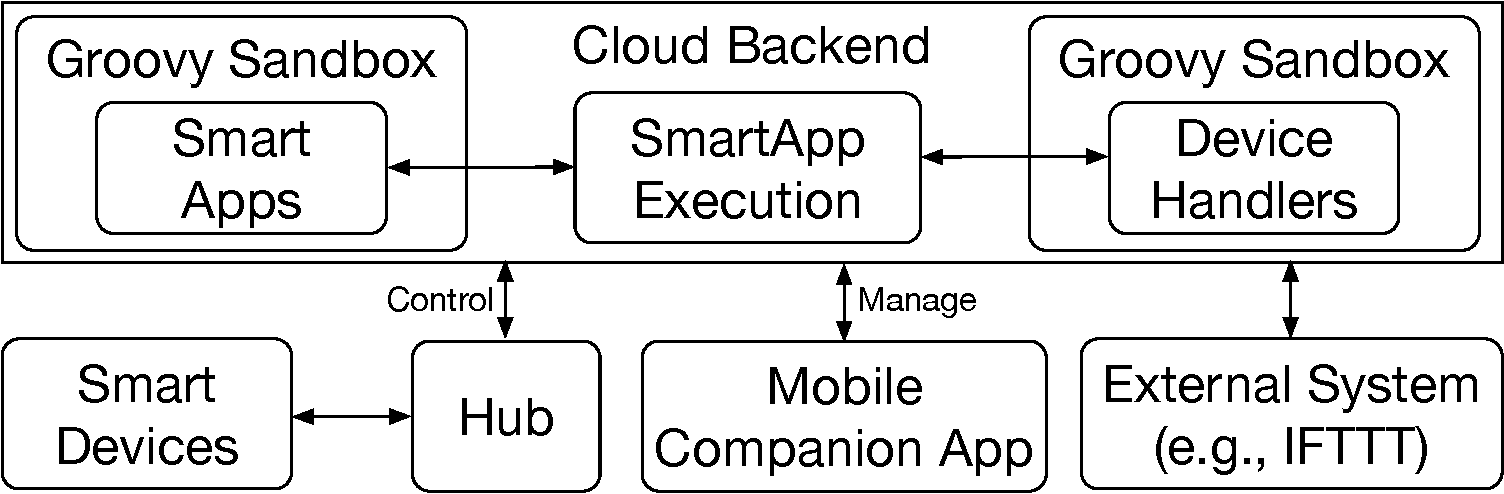
\includegraphics[width=3.0in]{SmartThingsArchitecture}
%\vspace{-0.1in}
\caption{SmartThings architecture overview.}
%\vspace{-.3in}
\label{SmartThingsArchitecture}
\end{center}
\end{figure}
%}
%\end{comment}

\subsection{Communications} {\color{black}ZigBee, which is build upon the PHY and MAC layers specified by IEEE 802.15.4, and Z-Wave, which adheres to the ITU-T G.9959 PHY and MAC layers, are among the most common wireless protocol stacks supported by an alliance of IoT product vendors \cite{Samsung:smartthingsproduct,Philips:hue,Yale:assurelock,Ecobee:thermostat}. Recent studies on link reliability of ZigBee and Z-Wave wireless networks have shown that one-hop retransmission is optionally supported by MAC layer and end-to-end retransmission is done by upper layers (\textit{e.g.}, application support sublayer) and depends on the implementation of the vendors \cite{s140814932,5747474,6379462,6392527,FULLER201744,7745306}.

Our study on communication protocols of Samsung SmartThings confirms that} the hub communicates with IoT devices using a protocol such as ZWave or ZigBee.
Experiments using the EZSync CC2531 Evaluation Module USB Dongle \cite{TI:CC2531} of
Texas Instruments, reveal that the ZigBee implementation
in SmartThings supports four (single hop) MAC layer retransmissions.
In addition, SmartThings has an application support sublayer that performs 15
end-to-end retransmissions (for a total of 60 retransmissions of a packet).
These are in line with ZigBee specifications as also verified in
\cite{s140814932,5747474,6379462,6392527}. Thus, typically,
it is rare that the system will transition to unsafe states because
of benign packet losses.


\begin{comment}
{
\thomas{ZigBee, which is build upon the PHY and MAC layers specified by IEEE 802.15.4, and Z-Wave, which adheres to the ITU-T G.9959 PHY and MAC layers, are among the most common wireless protocol stacks supported by an alliance of IoT product vendors \cite{Samsung:smartthingsproduct,Philips:hue,Yale:assurelock,Ecobee:thermostat}. Recent studies on link reliability of ZigBee and Z-Wave wireless networks have shown that one-hop retransmission is optionally supported by MAC layer and end-to-end retransmission is done by upper layers (\textit{e.g.}, application support sublayer) and depends on the implementation of the vendors \cite{s140814932,5747474,6379462,6392527,FULLER201744,7745306}. We have used the EZSync CC2531 Evaluation Module USB Dongle \cite{TI:CC2531} of Texas Instruments to evaluate the ZigBee communication protocols of Samsung SmartThings and found out that SmartThings' ZigBee supports four times of one-hop retransmissions and 15 times of end-to-end retransmissions. Therefore, we believe that SmartThings' ZigBee can guarantee end-to-end reliable transmission under normal conditions (\textit{e.g.}, without traffic jamming attacks) with the total number of 60 retransmissions.}
}
\end{comment}

\begin{comment}
{
\thomas{Many users have reported the failures of their ZigBee and Z-Wave IoT devices (\textit{e.g.}, motion sensors, water leak sensors, presence sensors, contact sensors, and garage door openers) in the SmartThings Community \cite{Samsung:smartthingscom1,Samsung:smartthingscom2, Samsung:smartthingscom3, Samsung:smartthingscom4}. Moreover, we have done some simple experiments to verify the behavior of the SmartThings system when device failure happens. The system under test comprises of a Samsung Hub, a Z-Wave smart lock, and a ZigBee smart power outlet. First, we unlocked the lock and turned on the outlet. As shown in the mobile companion app, the status of the lock was ``unlocked" and the status of the outlet was ``on". Second, we removed the battery of the lock and unpluged the outlet from the power strip. It took the mobile companion app about 12 minutes and 60 minutes to mark the outlet and the lock as ``unavailable'', but the status of the outlet was still ``on" and status of the lock was still ``unlocked". Even though the devices already stopped working, it took the SmartThings a long time to notify the failure to the users. During that time, an IoT system may enter bad states. Therefore, we need to take into account device failures when verifying IoT systems.}
}
\end{comment}

%\vspace{-.15in}
%\section{Misconfiguration Problems}
\section{Motivating Examples}
\label{sec:motivation}
{\color{black}We use two examples of violations found via our experiments (more details in \S~\ref{sec:eval}) to motivate our work.
Although simple, these examples exemplifies the safety problems that arise with third party IoT apps.

\subsection{Unsafe Physical States} In this example, a user installs three smart apps viz., \textit{Light Off When Close}, \textit{Good Night},
and \textit{Big Turn Off} to automate her smart home.
\textit{Light Off When Close} will turn off
configured lights when the configured contact sensor detects door closing;
\textit{Good Night} will change the location mode to \textit{Sleeping}
when all the monitored lights and motion sensors are inactive for
a configured period during night; and
\textit{Big Turn Off} will turn off all the configured devices
when (i) the user touches the app or (ii) the app detects a location mode change.

If we define a safety property as
\textit{temperature should always be higher than 0 degree Celsius},
a violation instance can be discovered by \sys as follows.
At night, after the owner closes the door monitored by
the \textit{Light Off When Close} app, it turns off the lights.
After a while, the app \textit{Good Night} changes the location mode to \textit{Sleeping}.
Upon the location mode change, \textit{Big Turn Off} turns off all of the configured devices,
which includes a heater.
Because the temperature can be below 0 degree during night,
this can lead to a violation of our safety property.

The violation scenario can be avoided if
(i) \textit{Big Turn Off} turns off the configured devices \emph{only} when the user touches the app,
(ii) \textit{Big Turn Off} explicitly asks users to configure that the configured devices to be turned off
only upon transitioning to a specific mode (\eg, ``Away''),
(iii) \textit{Big Turn Off} is installed together with only apps that change
the location mode to ``Away" when people leave home,
or (iv) \textit{Big Turn Off} is not configured to the heater.
Unfortunately, the first three options are not feasible and users may
have valid reasons to configure the app to control the heater.}

\subsection{Misconfiguration Problems} Besides malicious apps, misconfiguration is a common cause for safety violations.
When installing a smart app, a user has
to configure the app with sensor(s) and actuator(s). Poor configurations
can transition the IoT system to unsafe physical states.
There are many common causes for such misconfigurations, \eg,
(i) the app's description is unclear,
(ii) there are too many configuration options,
and (iii) normal users often do not have good domain knowledge to
clearly understand the behaviors of smart devices and smart apps.
To exemplify these issues, we conduct a user study (more details in \S\ref{sec:eval})
where we asked 7 student volunteers to configure various apps as they deemed fit.
Among these apps, one app is called \textit{Virtual Thermostat} and describes itself as
``Control a space heater or window air conditioner (AC) in conjunction with any temperature sensor, like a SmartSense Multi.''
{\color{black}Figure~\ref{inputexample} shows the inputs needed from a user,
which include a temperature measurement sensor (lines 2-4),
the power outlets into which the heater or the AC are plugged (lines 5-7),
a desired temperature (lines 8-10), etc.}
Although the developers use the word {\em or} and the app only expects
either a heater or an AC,
5 out of 7 student volunteers thought the app controls {\em both}
a heater and an AC to maintain the desired temperature and
mis-configured the app to control both the AC outlet and the heater outlet.
To exacerbate the confusion, the app expects
the configuration of outlets (\texttt{capability.switch})
instead of the actual devices that are plugged into the outlets
(\ie, AC or heater) (note that the SmartThings UI displays all available outlets to the user).
As a result of volunteer misconfigurations, when the temperature is higher than a predefined threshold,
the \textit{Virtual Thermostat} would turn on both the configured outlets
(\ie, both the heater and the AC).
This violates the following two commonsense properties:
(i) a heater is turned on when temperature is above a predefined threshold and
(ii) an AC and a heater are both turned on.

\begin{figure}[tb]
%\scriptsize
%\tiny
\begin{center}
\ssp
\lstinputlisting[language=groovy]{./code/virtualthermostat.groovy}
%\vspace{-0.17in}
\caption{{\color{black}Example of input info needed from users to configure the app \textit{Virtual Thermostat}.}}
\label{inputexample}
\end{center}
%\vspace{-0.22in}
\end{figure}

{\color{black}While these examples are quite simple, it exemplifies an important problem:
it is very possible that users may not carefully evaluate their IoT systems so
it can be driven into bad states,
especially when apps are installed or configured at different times
or by different users.
In practice, it is also difficult for typical users who do not have a strong
technical background to assess if bad interactions are possible.
Even if cursory examinations reveal simple violations,
complex violations are harder to find manually.
The latter is true especially if such interactions result from a chain of
sensing and actuation events across multiple devices controlled
by independent apps.
Thus, an automated way of discovering such bad interactions is necessary.}

\begin{comment}
\begin{figure}[tb]
\begin{center}
\includegraphics[width=3.0in]{inputexample}
%\vspace{-0.1in}
\caption{{\color{black}Example of input info needed from users to configure the app \textit{Virtual Thermostat}.}}
\label{inputexample}
\end{center}
%\vspace{-0.25in}
\end{figure}
\end{comment}


%\vspace{-0.14in}
\section{Model Checking as a Building Block}
The problem of reasoning if and why the IoT system
could transition into a bad physical state
is challenging because the number of apps and devices is likely to
grow in the future and thus, analyzing all possible interactions
between them will be hard.
Static analysis tools tend to sacrifice completeness for soundness,
and thus result in lots of false positives.
In contrast, typical dynamic analyses tools
verify the properties of a program during execution,
but can lead to false negatives.

Model checking is a technique that checks
whether a system meets a given specification~\cite{jhala2009software},
%In software model checking~\cite{jhala2009software},
%the system is a program and specifications are safety and liveness properties.
by systematically exploring the program's state.
In an ideal case, the model checker exhaustively examines all possible system states to verify
{\color{black}if there is any violation} of specifications relating
to safety and/or liveness properties.
%However, the undecidability of the halting problem implies that for
%complex systems such as IoT, neither 
%general analysis algorithm that can be both sound and complete.
\textcolor{black}{However, the complexity of modern system software makes this extremely challenging computationally.}
So in practice, when the goal is to find bugs, a model checker is usually
used as a \emph{falsifier} \ie, it explores a portion of the reachable state
space and tries to find a computation that violates the specified property.
This is sometimes
also called bounded model checking~\cite{Biere1999:BMC, Kroening2014:CBMC, Merz2012:LLBMC, Cordeiro2012:ESBMC,Roya:networkprotocol}.

We adopt model checking as a basic building block since:
(i) it provides the flexibility towards verifying
all the desired properties with linear temporal logic\footnote{
  Linear temporal logic (LTL) is
  a modal temporal logic with modalities referring to time.
  LTL is used to verify
  properties of reactive systems~\cite{Baier:modelchecking}.},
(ii) it provides concrete counter-examples~\cite{Baier:modelchecking,Spin:intro}
which are very useful in analyzing why and how the bad states occur,
(iii) its holistic nature of checking can capture interactions among multiple apps,
and (iv) it is more efficient than exhaustive testing \cite{10.1007/978-3-319-70389-3_7}.
%
However, a successful model checker must address the state explosion problem,
\ie, the state space could become unwieldy and requires exponential time to explore.

%\begin{comment}
{\color{black}Model checking can be grouped into two classes:
(a) explicit model checking~\cite{Clarke1982} where progress is made one state at a time and,
(b) symbolic model checking~\cite{McMillan1993} that examines sets of states in each step.
Literature suggests that neither is a clear winner 
with regards to yielding complete verification within reasonable times
in all settings~\cite{Avrunin2000:benchmarking,Eisner2002:comparing,Holzmann1999:iprotocol}.

In brief, symbolic model checking is considered to perform better for synchronous hardware systems
and explicit model checking is better for concurrent software systems
\cite{Flavio2003:symbolicmodelchecking,Choi2007:nusmvtospin,Dong1999:fighting}.
Biere~\etal, claim that explicit model checking is the most efficient model checking technique in practice
if the number of reachable states is small, \ie,
below several million states~\cite{Armin2001:verifyingsequentialbehavior}.
Eisner~\etal argue that a symbolic model checker performs better even for
asynchronous systems~\cite{Eisner2002:comparing}.
However, there are other reports that indicate that a
direct comparison of the two categories is almost impossible
\cite{Avrunin2000:benchmarking,Eisner2002:comparing,Holzmann1999:iprotocol}.}
%
%}
%\end{comment}

{\color{black}Given its popularity and flexibility in modelling both concurrent and synchronous systems \cite{Flavio2003:symbolicmodelchecking,Choi2007:nusmvtospin,Dong1999:fighting}, we use \spin~\cite{Holzmann:spin} for checking if a given set of safety properties can be possibly violated.}
%Specifically, we use the popular \spin model checker~\cite{Holzmann:spin} for
%checking if a given set of safety properties can be possibly violated.
%\spin is a popular open-source software model checking tool,
%used for the formal verification of multi-threaded software applications.
Since an IoT system may be composed of a large number of apps and smart devices,
we use \spin's verification mode with BITSTATE hashing---an approximate technique
that stores the hash code of states in a bitfield instead of storing the whole states.
Although the BITSTATE hashing technique does not provide a complete verification,
empirical results and theoretical analysis have proved its effectiveness
in terms of state coverage
\cite{Holzmann1998,Cattel94,Chaves91,Holzmann94:NewCoRe,Holzmann94:prove}.

\chapter{Scope and Threat Model}
%\section{Scope and Threat Model}
In this work, our goal is to detect safety issues (\ie, vulnerabilities) of IoT systems
that are exploitable by attackers to transition the system 
into bad physical states or leak sensitive information.
Safety requirements (\ie, definition of bad states and information leakage)
can come from both the users and security experts.
Examples of bad physical states are
(i) the front door is unlocked when no one is at home,
and (ii) a heater is turned off when the temperature is
{\color{black}below a predefined threshold}.
%An example of a bad cyber state is the leakage of the users' sensitive data.
%The safety properties with regards to
{\color{black} With regards to information leakage we require that:
(i) private information is sent out via only message interfaces
(\eg, \textit{sendSmsMessage} and \textit{sendPushMessage} in SmartThings) but not
via network interfaces (\eg, \textit{httpPost} in SmartThings), and
(ii) the recipients of methods for sending messages match the configured phone numbers or contacts.
We point out that legitimate apps might use network interfaces to
send some control information (\eg, relating to crashes) back to the server.}
In such cases, we assume that users dictate whether to allow/disallow such operations
(based on their privacy preferences).
%In other words, we let the user decide which properties their IoT system must satisfy.}
%are within the family members.

We consider all devices (hub, sensors, and actuators), the cloud, and the companion app
as our trusted computing base (TCB), and do not consider software attacks against them.
However, \sys does mitigate physical attacks that can inject event(s) into the system
(\eg, by physically increasing the temperature or spoofing the sensors)
or maliciously induced device or communication failures (\eg, by jamming~\cite{5473884}).
\sys seeks to identify and prevent such events from leading the system into safety violations.
However,  targeted solutions to those attacks
(\eg, preventing spoofing of sensors or jamming mitigation) are out-of-scope.

We also consider potential bad states that can arise
due to natural device failures.
Note that many users have reported the failures of their ZigBee and Z-Wave IoT devices
(\textit{e.g.}, motion sensors, water leak sensors, presence sensors, and garage door openers)
in the SmartThings Community~\cite{Samsung:smartthingscom1,Samsung:smartthingscom2, Samsung:smartthingscom3, Samsung:smartthingscom4}.
Failures could also result from device batteries running out.
We seek to identify if such device failures can cause an IoT system to transition
into a bad physical state.

%Apps can be benign but vulnerable or malicious.
Malicious apps can exploit weaknesses in the configuration and
attack other apps by introducing problematic events.
We only seek to attribute an app as possibly malicious and
leave the {\color{black}confirmation} to human experts or other systems.

\begin{comment}
{
\section{Motivating Examples}
\label{sec:motivation}

We use two examples of violations found via our experiments (more details in \S~\ref{sec:eval}) to motivate our work.
Although simple, these examples exemplify the safety problems that arise with third party IoT apps.

\textbf{First Example:} a user installs three smart apps viz., \textit{Light Off When Close}, \textit{Good Night},
and \textit{Big Turn Off} to automate her smart home.
\textit{Light Off When Close} will turn off
configured lights when the configured contact sensor detects door closing;
\textit{Good Night} will change the location mode to \textit{Sleeping}
when all the monitored lights and motion sensors are inactive for
a configured period during night; and
\textit{Big Turn Off} will turn off all the configured devices
when (i) the user touches the app or (ii) the app detects a location mode change.

If we define a safety property as
\textit{temperature should always be higher than 0 degree Celsius},
a violation instance can be discovered by \sys as follows.
At night, after the owner closes the door monitored by
the \textit{Light Off When Close} app, it turns off the lights.
After a while, the app \textit{Good Night} changes the location mode to \textit{Sleeping}.
Upon the location mode change, \textit{Big Turn Off} turns off all of the configured devices,
which includes a heater.
Because the temperature can be below 0 degree during night,
this can lead to a violation of our safety property.

The violation scenario can be avoided if
(i) \textit{Big Turn Off} turns off the configured devices \emph{only} when the user touches the app,
(ii) \textit{Big Turn Off} explicitly asks users to configure that the configured devices {\color{black}to be} turned off
only upon transitioning to a specific mode (\eg, ``Away''),
(iii) \textit{Big Turn Off} is installed together with only apps that change
the location mode to ``Away" when people leave home,
or (iv) \textit{Big Turn Off} is not configured to the heater.
Unfortunately, the first three options are not feasible and users may
have valid reasons to configure the app to control the heater.


\thomas{\textbf{Second Example:} a user installs two smart apps viz., \textit{Away Mode With Eco Turn Off} and \textit{Lock Down} to automate her smart home.
\textit{Away Mode With Eco Turn Off} will change location mode to \textit{Away} when all people leave home and turn off some devices; and
\textit{Lock Down} will lock all the configured locks when (i) the user touches the app or (ii) the app detects a location mode change.}

\thomas{If we define a safety property as
\textit{The entrance door must be locked when all people leave home}, a violation instance can be discovered by \sys as follows.
When all people leave home (\textit{i.e.}, states of all presence sensors change to ``not present''), \textit{Away Mode With Eco Turn Off} changes location mode to \textit{Away}. Upon the location mode change, \textit{Lock Down} sends the ``lock'' command to the entrance door. Unluckily, the entrance door is offline/unavailable at that time and thus is not locked. Similarly, the defined property will be also violated when one of the presence sensors goes offline (assume that its last state is ``present''). As a result, when all people leave home, \textit{Away Mode With Eco Turn Off} will not change location mode to \textit{Away} and thus \textit{Lock Down} is not triggered to lock the entrance door.}

\thomas{Many users have reported the failures of their ZigBee and Z-Wave IoT devices (\textit{e.g.}, motion sensors, water leak sensors, presence sensors, contact sensors, and garage door openers) in the SmartThings Community \cite{Samsung:smartthingscom1,Samsung:smartthingscom2, Samsung:smartthingscom3, Samsung:smartthingscom4}. Therefore, we should definitely consider the impact of device failures on IoT systems.}

While these examples are quite simple, they exemplify an important problem:
it is very possible that users may not carefully evaluate their IoT systems so
it can be driven into bad states,
especially when apps are installed or configured at different times
or by different users.
In practice, it is also difficult for typical users who do not have a strong
technical background to assess if bad interactions are possible.
Even if cursory examinations reveal simple violations,
complex violations are harder to find manually.
The latter is true especially if such interactions result from a chain of
sensing and actuation events across multiple devices controlled
by independent apps.
Thus, an automated way of discovering such bad interactions is necessary.
}
\end{comment}

%\vspace{-0.11in}
\chapter{System Overview}\label{overview}
\section{Chain of Events in an IoT System}
Figure~\ref{chainreaction} illustrates a high level view of the chain of events in an IoT system.
In brief, sensors sense the physical world and convert them into events in the cyber world;
these events, in turn, are passed onto apps that subscribe to such events.
Upon processing the cyber events these apps may
output commands to actuators, which
then trigger new physical or cyber events.
Apps may also directly generate new cyber events.
Therefore, a single event could lead to a large sequence of subsequent cyber/physical events.
%which could translate to a large state space to check.

\begin{figure}[tb]
\begin{center}
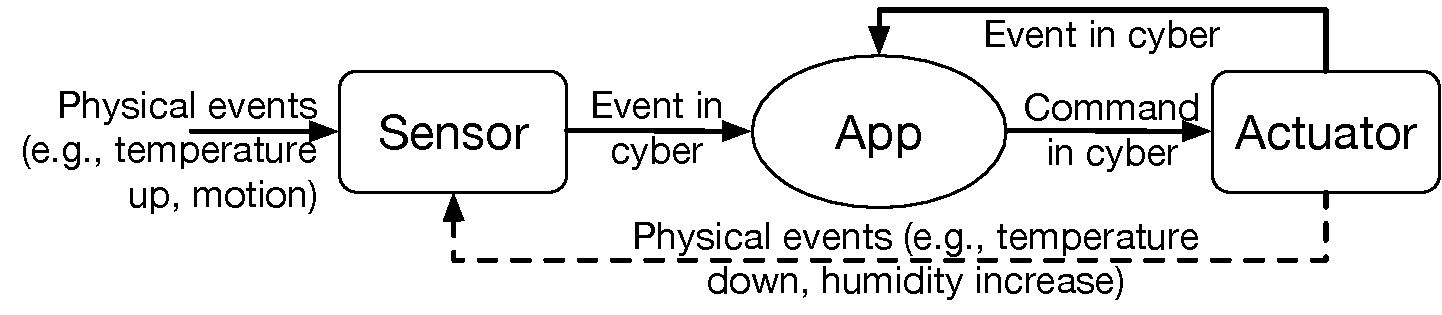
\includegraphics[width=3.5in]{chainreaction}
%\vspace{-0.17in}
\caption{Chain of events in an IoT system.}
\label{chainreaction}
\end{center}
%\vspace{-0.23in}
\end{figure}

%Moreover, state change events of actuators may trigger some apps \thomas{Do we need to talk about the permutation of input events here}. Therefore, with a single physical event, there may be many events generated in the cyber world. That is, the state space may get exponentially exploded with just a small amount of input physical events.

\section{Overall Architecture}
Figure~\ref{iSanitizerArchitecture} depicts the architecture of our system \sys.
It consists of five modules viz.,
\textit{App Dependency Analyzer}, \textit{Translator}, \textit{Configuration Extractor}, \textit{Model Generator}, and \textit{Output Analyzer}.
In designing \sys, we tackle two main challenges:
(i) alleviating the state space explosion with model checking~\cite{Clarke2012} for our context, and
(ii) the translation of smart apps' source code to Promela (to facilitate model checking).
We address the first problem partially in the \textit{App Dependency Analyzer}
and partially in the \textit{Model Generator}.
The second problem is handled partially in the \textit{Translator}
and partially in the \textit{Model Generator}.

\begin{figure}[tb]
\begin{center}
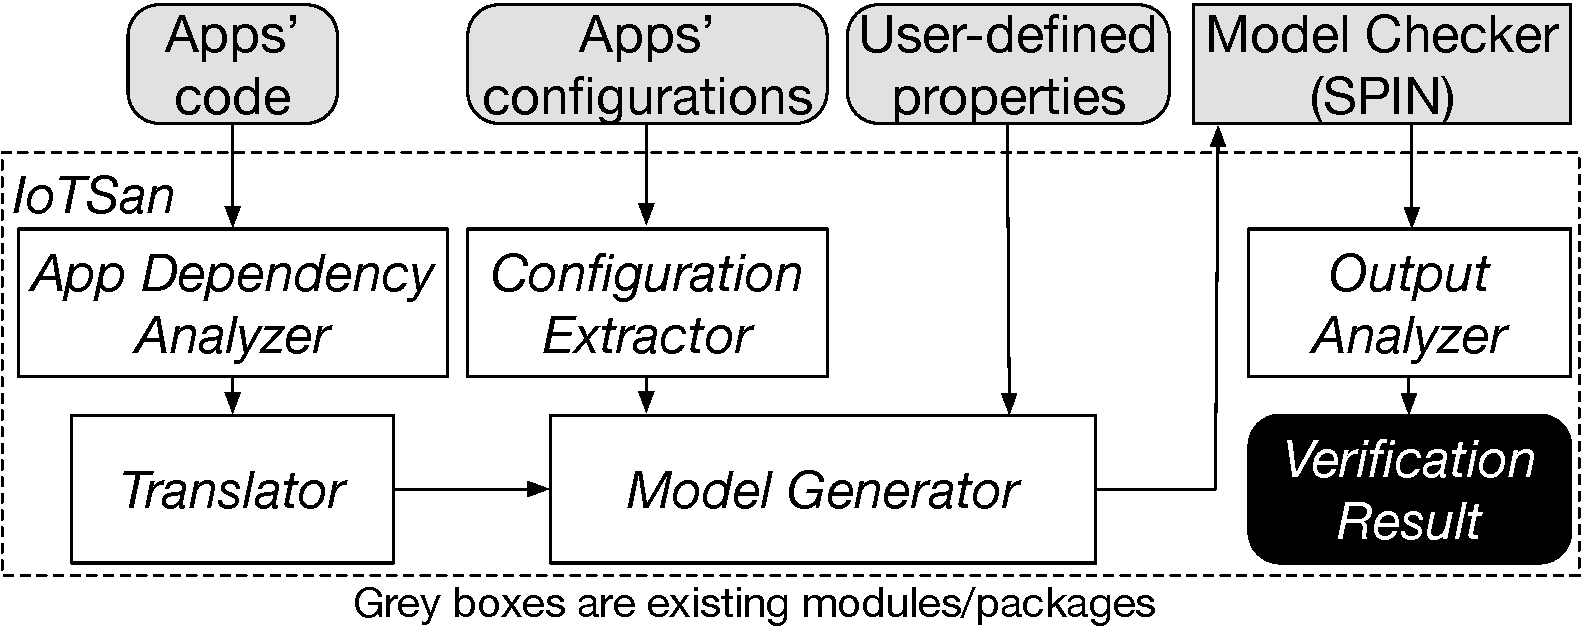
\includegraphics[width=3.1in]{iSanitizerArchitecture}
%\vspace{-0.1in}
\caption{\sys architecture overview.}
\label{iSanitizerArchitecture}
\end{center}
%\vspace{-0.25in}
\end{figure}

\textbf{\em App Dependency Analyzer} (\S~\ref{sec:depedency}):
This module constructs dependency graphs to capture
interactions between {\color{black}event handlers of different apps
and identifies handlers that must be jointly analyzed by the model checker.
This precludes the unnecessary analysis of unrelated event handlers.}
%Then, we verify only the apps in the same dependent set together while excluding other unrelated apps.

\textbf{\em Translator} (\S~\ref{sec:translator}):
%To the best of our knowledge, there are no model checking systems that readily verify Groovy programs.
We build a translator within \sys, that automatically converts Groovy programs into Promela.
In doing so, we address the following challenges:
\begin{itemize}
\item {\em Implicit Types}. In Groovy programs, data types of variables and return types of functions are not
explicitly declared. To solve this problem, we design an algorithm to infer data types of variables and return types of functions.
%\krish{People frown at heuristics. Can we say something else - or at least why this is good ?} \thomas{I have changed it to \textit{context-based}}
\item {\em Built-in Utilities}. Groovy has many built-in utilities,
\textit{e.g.}, \texttt{find}, \texttt{findAll}, \texttt{each}, \texttt{collect},
\texttt{first}, $+$ on list types, and \texttt{map}.
We manually analyzed the behavior of each utility and translated them into corresponding code in Promela.
%\krish{I don't think we should say "we have to". Did we do this ? Was this manual? This part is vague otherwise.} \thomas{We manually analyze the behaviors but the translation process is automatic.}
\end{itemize}
%The \textit{Translator} module outputs the Promela code of apps' event handlers.

\textbf{\em Configuration Extractor} (\S~\ref{sec:extractor}):
IoT platforms often provide a companion mobile app and/or
web-based app to manage/configure the installed smart apps and devices of an IoT system.
This module automatically extracts the system's configurations from the manager app.
%It also gets a list of desired properties from the user.

\textbf{\em Model Generator} (\S~\ref{sec:model}):
This module takes the Promela code of event handlers,
the configuration of the IoT system, and safety properties (both pre-defined and user-defined) as inputs,
and creates the Promela model of the system.
We use sequential design to model the IoT system instead of concurrent design.
This significantly reduces the problem size by eliminating
unnecessary interleaving that is unlikely to yield useful assessment of unsafe behaviors.
The generated model is checked by \spin for possible property violations.

\textbf{\em Output Analyzer} (\S~\ref{outputanalyzer}):
This module analyzes the verification logs and attributes safety violations to potentially malicious apps,
bad designs or misconfiguration.
Based on the result, it provides the user, a suggestion to either remove a bad app(s) or change an app(s)'s
configuration.

%{\color{violet}Table~\ref{table:comparison} shows the comparison of \sys and related work (more details in \S~\ref{sec:related}).}

\begin{table}[t]
\scriptsize
\ssp
%\vspace{-0.12in}
\caption{Comparison of \sys and related work.}
%\vspace{-0.12in}
\label{table:comparison}
\centering
\begin{tabular}{| p{5cm} | c | c | c | c |}
\hline
\textbf{Feature} & \textbf{SIFT \cite{Liang:2015:SBI:2737095.2737115}} & \textbf{DeLorean \cite{190480}} & \textbf{Soteria \cite{215955}} & \textbf{\sys}\\
\hline
Detects physical safety violations & \Checkmark & \Checkmark & \Checkmark & \Checkmark\\
\hline
Detects information leakage &  &  &  &  \Checkmark\\
\hline
Detects violations due to communication/device failures &  &  &  &  \Checkmark\\
\hline
Detects violations due to misconfiguration problems &  &  &  &  \Checkmark\\
\hline
Handles complex code beyond IFTTT rules &  & \Checkmark & \Checkmark & \Checkmark\\
\hline
Performs violation attribution &  &  &  &  \Checkmark\\
\hline
%Targets legacy apps & \Checkmark & \Checkmark & \Checkmark &  & \Checkmark\\
%\hline
Accounts for app interactions & \Checkmark &  & \Checkmark & \Checkmark\\
\hline
%\textbf{No need for app patches} &  &  &  &  & \Checkmark\\
%\hline
%Platform compliant &  & \Checkmark &  & \Checkmark & \Checkmark\\
%\hline
\end{tabular}
%\vspace{-0.21in}
\end{table}

\begin{comment}
\begin{table}[t]
\scriptsize
%\vspace{-0.12in}
\caption{Comparison of \sys and related work.}
%\vspace{-0.12in}
\label{table:comparison}
\centering
\begin{tabular}{| p{1.9cm} | p{1.05cm} | p{1.12cm} | p{1.15cm} | p{0.45cm} | p{0.6cm} |}
\hline
\textbf{Feature} & \textbf{SIFT \cite{Liang:2015:SBI:2737095.2737115}} & \textbf{DeLorean \cite{190480}} & \textbf{Soteria \cite{215955}} & \textbf{SIFT \cite{Liang:2015:SBI:2737095.2737115}} & \textbf{\sys}\\
\hline
\textbf{Detects physical safety violations} & \Checkmark & \Checkmark & \Checkmark & \Checkmark & \Checkmark\\
\hline
\textbf{Detects information leakage} &  &  &  &  & \Checkmark\\
\hline
\textbf{Detects violations due to communication failures} &  &  &  &  & \Checkmark\\
\hline
\textbf{Detects violations due to misconfiguration problems} &  &  &  &  & \Checkmark\\
\hline
\textbf{Handles complex code beyond IFTTT rules} &  & \Checkmark & \Checkmark & \Checkmark & \Checkmark\\
\hline
\textbf{Performs violation attribution} &  &  &  &  & \Checkmark\\
\hline
%Targets legacy apps & \Checkmark & \Checkmark & \Checkmark &  & \Checkmark\\
%\hline
\textbf{Accounts for app interactions} &  &  &  & \Checkmark & \Checkmark\\
\hline
%\textbf{No need for app patches} &  &  &  &  & \Checkmark\\
%\hline
%Platform compliant &  & \Checkmark &  & \Checkmark & \Checkmark\\
%\hline
\end{tabular}
%\vspace{-0.1in}
\end{table}
\end{comment}

%\subsection{Overall Architecture}
%Figure \ref{iSanitizerArchitecture} shows the overall architecture of our proposed system - \sys. The input of our system, which comprises of smart apps' source code and their configurations from users, goes into the \textit{App Dependency Analysis}, whose output are sets of dependent apps. The apps in each dependent set are fed into the \textit{Translator}. The result of the \textit{Translator} is in form of an intermediate representation (IR), \textit{e.g.}, Jimple. The \textit{Model Generator} takes apps' IR and configurations as inputs, and then creates a model in the target language of the model checker. In this paper, we use Spin for the model checker. Thus, the result of \textit{Model Generator} is  a Promela model, which is then verified by the Spin model checker. The verification result is checked by the \textit{Output Analyzer}. If detecting any violation, \textit{Output Analyzer} will attribute it to either bad app or bad configuration. The final result given to users is either (ii) no violation or (ii) suggestion to either remove some bad apps or change apps' configuration.

% \textbf{User Inputs}: \textcolor{black}{Upon installation, a user needs
% to configure a smart
% app. Poor configurations
% may cause the IoT system to transition to unsafe physical states.
% There are many common causes for such configurations. These are: (i) the app's description is not clear or misleading, (ii) there are too many configuration options, and (iii) normal users often do not have good domain knowledge to clearly understand the behaviors of smart devices and smart apps. To exemplify these issues, consider the following example. Figure \ref{inputexample} shows the input info that the app \textit{Virtual Thermostat} needs
% from a user. First, the description of the app is vague and states ``Control a space heater or window air conditioner (AC) in conjunction with any temperature sensor, like a SmartSense Multi."  \textit{Virtual Thermostat} asks users to configure a
% temperature measurement sensor (lines 2-5), the {\color{black} power} outlets into
% which the heater and the AC are plugged into (lines 6-9), a desired temperature (lines 10-12),
% etc.
% This seems to suggest that the app controls {\em both} the heater and the AC
% to maintain the desired temperature; however, it only expects one type of device.
% Second, since power outlets are used to control many type of devices (\textit{e.g.}, smart bulb, TV, AC, and heater), the SmartThings displays (exports) all of the outlets (capability.switch) in the IoT system to the user; in other words
% there are too many configuration options provided to the user.
% }

% %\krish{Did we discuss the user study before at all, it comes abruptly -- and we don't say why we do this. Should we say this somewhere earlier?}
% Finally, to showcase (iii)
% we conduct a user study (more details in \S~\ref{sec:eval})
% where we asked 7 student volunteers to configure various apps as they deemed fit.
% In this case, 5 out of 7 student volunteers configure the app to control both the AC and the heater (which it is not equipped to do). This caused the following. \textcolor{black}{When the temperature is higher than a predefined threshold, the \textit{Virtual Thermostat} turned on both the configured outlets, \textit{i.e.}, both the heater and the AC are turned on!
% As evident, this violates the following two
% commonsense properties: (i) a heater is turned on when temperature is {\color{black}above a predefined threshold}, and (iii) an AC and a heater are both turned on.}
% %\textcolor{red}{Note that we may have problem only when an AC and a heater in the same room/house are both turned on, \textit{i.e.}, this may not be a violation if the two devices are at different locations; and we let the user decide which properties their IoT system should satisfy.}

\section{Our Work in Perspective} \sys can be envisioned as a service 
that jointly considers the apps, devices and their configurations of an IoT system, and checks whether a set of a priori defined properties hold. In addition to detecting safety violations of the physical space, it also detects information leakage. {\color{black}
Finally, it also determines if communication/device failures can cause unsafe states and detects violations due to misconfiguration problems}. In Table~\ref{table:comparison} we show the features that
\sys offers compared to the most related recent systems. A discussion of related work is deferred to \S~\ref{sec:related}.

%\vspace{-0.12in}
\chapter{App Dependency Analyzer}
\label{sec:depedency}
\begin{comment}
{
\section{Overview}
Each smart app can subscribe to events generated by one or more devices. In each subscription, the smart app provides a call back function (\textit{i.e.}, event handler) to SmartThings. Upon the occurrence of the subscribed event, SmartThings will trigger the registered event handler. Moreover, SmartThings also allows apps to register call back functions that will be triggered at some scheduled time. In summary, each smart app may have one or more event handlers. \textit{App Dependency Analysis} takes a set of event handlers of apps as inputs, build a dependency graph (DG), and calculating dependent sets. The event handlers in each dependent set need to be verified together since the inter-action among them may result in some violations. Moreover, the event handlers in different dependent sets may have conflicting behaviors, which may result in conflicting command violation. Therefore, the event handlers involving in a conflict also needs to be verified together.
}
\end{comment}

\begin{table}[bt]
\scriptsize
\ssp
\caption{An example to showcase the construction of a dependency graph.}
%\vspace{-0.12in}
\label{dgconstructiontb}
\centering
\begin{tabular}{| p{2.7cm} | l | p{1.5cm} | p{2.6cm} | p{2.5cm} |}
\hline
\bf App's Name & \bf Event Handler & \bf Vertex's ID & \bf Input Events & \bf Output Events\\
\hline
Brighten Dark Places & contactOpenHandler & 0 & contact/open, illuminance/``..." &  switch/on\\
\hline
Let There Be Dark! & contactHandler & 1 & contact/``..." &  switch/on, switch/off\\
\hline
Auto Mode Change & presenceHandler & 2 & presence/``..." &  location/mode\\
\hline
\multirow{2}{2.7cm}{Unlock Door}  & appTouch & 3 & app/touch & lock/unlocked\\ \cline{2-5}
	& changedLocationMode & 4 & location/mode & lock/unlocked\\
\hline
\multirow{2}{3cm}{Big Turn On}  & appTouch & 5 & app/touch & switch/on\\ \cline{2-5}
	& changedLocationMode & 6 & location/mode & switch/on\\
\hline
\end{tabular}
%\vspace{-0.13in}
\end{table}

%The first module of \sys determines sets of apps that are inter-dependent \textit{i.e.}, can jointly influence
%actuator actions. The reason for doing this is that,

The model checker should not have to check the interactions
between event handlers that do not interact. To find
event handlers that can interact and thus jointly influence actuator actions,
this module constructs a {\em dependency graph} (DG).
%This graph consists of
%{\em dependent sets} of apps \textit{i.e.}, sets of apps that interact either directly or indirectly.

\begin{comment}
{
\begin{figure}[t]
\begin{center}
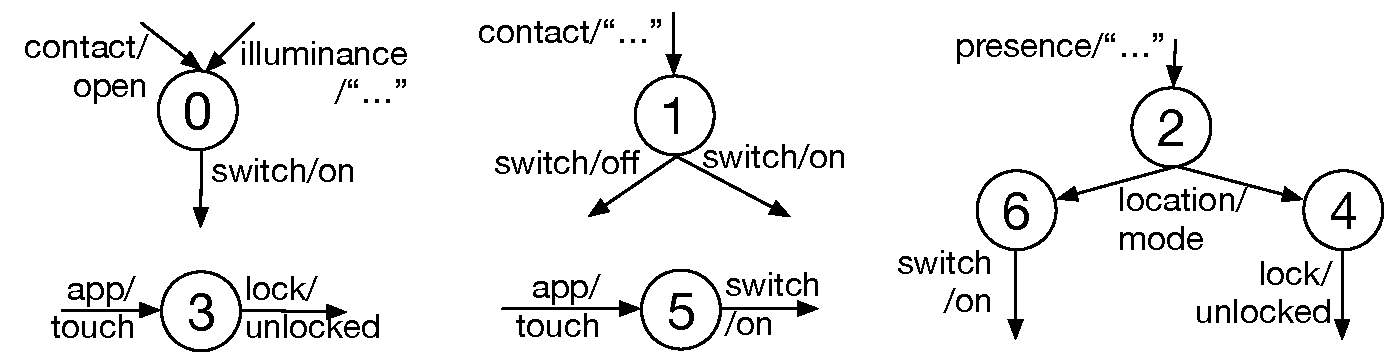
\includegraphics[width=3.0in]{DependencyGraphExample}
\vspace{-0.13in}
\caption{Example of a dependency graph.}
\label{dgconstructionfg}
\end{center}
\vspace{-0.33in}
\end{figure}
}
\end{comment}

\begin{figure}[bt]
    \centering
    \begin{subfigure}[t]{3.5in}
        \centering
        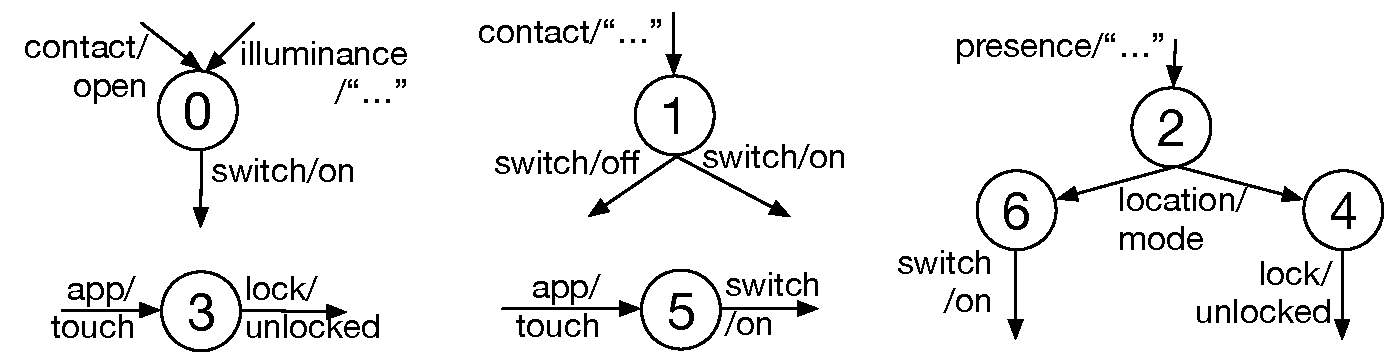
\includegraphics[width=3.5in]{DependencyGraphExample}
				%\vspace{-0.22in}
		\caption{Dependency graph.}
        \label{dgconstructionfg}
    \end{subfigure}\\
    \vspace{0.05in}
    \begin{subfigure}[t]{3.3in}
        \centering
        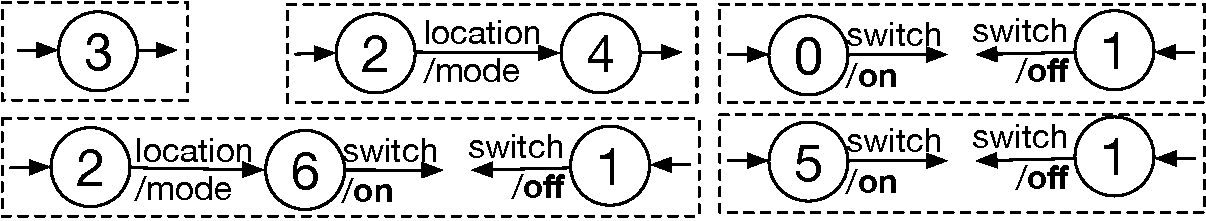
\includegraphics[width=3.3in]{related_set}
				%\vspace{-0.22in}
        \caption{\textcolor{black}{Related sets (each box represents a related set).}}
		%\vspace{-0.15in}
        \label{relatedset}
    \end{subfigure}
    \caption{Example of a dependency graph and its corresponding related sets.}
%\vspace{-0.25in}
\end{figure}

\section{Extracting Input/Output Events}
{\color{black}Each smart app registers one or more {\em event handlers} that get notified of events to
which it has subscribed.
%\zhiyun{each smart app has only one callback function? If so, maybe we should just say each vertex is an app to be more clear.}\thomas{No, one app may have several callback functions.}
An event handler takes one or more input events, and can induce zero or more output events.
Input events are (i) explicitly declared in the \texttt{subscribe} commands or,
(ii) identified via APIs that read states of smart devices,
or (iii) indicated by interrupts at specific times defined by \texttt{schedule} method calls.
Output events are invoked via APIs that change states of smart devices.

{\color{black}We enumerate the input and output events of an app using static analysis
%(details are straightforward and are omitted to save space).}
as follows. First, we parse and identify
all the read and write APIs in each function of the smart app. Second, we build call sequences whose entry points are event handlers. The input events of an event handler are identified by (i) the read APIs in its call sequence, (ii)
the events specified in its \textit{subscribe}, and times in its \textit{schedule} method calls.
The output events are identified by the write APIs in its call sequence.}

\section{Dependency Graph Construction}
\begin{comment}
Each smart app registers one or more {\em event handlers} that get notified of events to
which it has subscribed.
%\zhiyun{each smart app has only one callback function? If so, maybe we should just say each vertex is an app to be more clear.}\thomas{No, one app may have several callback functions.}
An event handler takes one or more input events, and can induce zero or more output events.
Input events are (i) explicitly declared in the \texttt{subscribe} commands or,
(ii) identified via APIs that read states of smart devices,
or (iii) indicated by interrupts at specific times defined by \texttt{schedule} method calls.
Output events are invoked via APIs and change states of smart devices.
We enumerate the input and output events of an app using static analysis
(details are straightforward thus omitted due to space constraints).
%as follows. First, we parse and identify
%all the read and write APIs in each function of the smart app. Second, we build call sequences whose entry points are event handlers. The input events of an event handler are identified by (i) the read APIs in its call sequence, (ii)
%the events specified in its \textit{subscribe}, and times in its \textit{schedule} method calls.
%The output events are identified by the write APIs in its call sequence.
\end{comment}
Once the input and output events are identified,
we construct a directed DG as follows.
Each event handler is denoted by a vertex in the DG.
An edge from a vertex $u$ to a vertex $v$ ($u \rightarrow v$) is added
if the output events of $u$ overlap with the input events of $v$.
$u$ is then called the \textit{parent} vertex of the \textit{child} vertex $v$.
The vertices in a strongly connected component are merged into a composite vertex (a union of input and output events).
A \textit{leaf} vertex does not have any child.

\section{Example}
To illustrate, consider the following example.
Table~\ref{dgconstructiontb} summarizes the event handlers and the associated input/output
events with a set of sample smart apps.
The description of an event is in the format \textit{attribute}/\textit{event type}
(\eg, contact/open means ``a contact sensor is open");
empty quotes (``...") denote ``any" event of that type.
Given these apps, we show the DG that is built in Figure~\ref{dgconstructionfg}.
For each vertex, the incoming arrows denote input events and the outgoing arrows denote output events.
For example, vertex $2$ has two children viz., vertex $4$ and vertex $6$; all vertices except vertex $2$ are leaf vertices.

%\section{Dependency Analysis}
%\subsection{Calculating dependent sets}
%As per the description of the DG construction, we can see that the behavior of a vertex $u$ (an event handler) in the DG depends on only its parents since the output events of its parents are some of or all of its input events. The behavior of the parents also depend on their own parents, and so on and so forth. Therefore,

{\bf \textcolor{black}{Related sets}:}
The initial {\em related set} of a leaf vertex $v \in$ DG includes all of its ancestors and $v$ itself.
There is no need to find such related sets for vertices that are not leaves,
since those sets are subsets of other leaves' related sets.
Table~\ref{dependentset} shows the
initial related sets in the DG from Figure~\ref{dgconstructionfg}.

\begin{table}[tb]
\scriptsize
    \caption{Related sets of the dependency graph in Figure \ref{dgconstructionfg}: (a) Initial related sets, (b) Potential conflicting sets, and (c) Final related sets.}
	%\vspace{-0.12in}
    \centering
    \begin{subtable}[t]{.32\linewidth}
      \centering
        \caption{}
		%\vspace{-0.05in}
        \label{dependentset}
	{
        \begin{tabular}{| c | l |}
	\hline
	\bf Set & \bf Vertexes\\
	\hline
	1 & 0\\
	\hline
	2 & 1\\
	\hline
	3 & 3\\
	\hline
	4 & 5\\
	\hline
	5 & 2, 4\\
	\hline
	6 & 2, 6\\
	\hline
	\end{tabular}
	}
    \end{subtable}%
    \begin{subtable}[t]{.32\linewidth}
      \centering
        \caption{}
		%\vspace{-0.05in}
        \label{dependentsetconflict}
	{
        \begin{tabular}{| c | l |}
	\hline
	\bf Set & \bf Vertexes\\
	\hline
	1 & 0, 1\\
	\hline
	2 & 1, 5\\
	\hline
	3 & 1, 2, 6\\
	\hline
	\end{tabular}
	}
    \end{subtable}
    \begin{subtable}[t]{.32\linewidth}
    \centering
        \caption{}
		%\vspace{-0.05in}
        \label{finaldependentset}
	{
    	\begin{tabular}{| c | l |}
	\hline
	\bf Set & \bf Vertexes\\
	\hline
	1 & 3\\
	\hline
	2 & 2, 4\\
	\hline
	3 & 0, 1\\
	\hline
	4 & 1, 5\\
	\hline
	5 & 1, 2, 6\\
	\hline
	\end{tabular}
	}
    \end{subtable}
%\vspace{-0.24in}
\end{table}

\hfill \break

The initial related sets constructed as above are incomplete.
This is because, two vertices
$u$ and $v$ may have common output events but the types of these events could be different or what we call
{\em conflicting}.
For example, nodes 0 and 1 have conflicting output events viz., switch/off and switch/on.
In such cases,
the related sets to which $u$ and $v$ belong, must be merged to account for such conflicts.
Table~\ref{dependentsetconflict} shows the related sets of vertices with potential output conflicts
in our example.
Note here that to check for such output conflicts, we need to examine $O(E^2)$ links in the worst case (given $E$ output edges from the event handlers);
our experiments show that such checks are very fast.

We point out that if a related set $i$ is a subset of a bigger related set $j$,
the model checker automatically verifies $i$ when $j$ is verified;
thus, there is no need to re-verify $i$.
In Table~\ref{finaldependentset} and Figure~\ref{relatedset},
we show the final related sets associated with the DG in Figure~\ref{dgconstructionfg}
after removing all redundant subsets.
These related sets are jointly analyzed by the model checker.

%\vspace{-0.23in}
\chapter{Translator}
\label{sec:translator}
{\color{black}Given its popularity and ease of use \cite{Shankar2018,Godefroid2018,Thomsen2015,Groce2014}}, we build \sys using the Bandera Tool Set \cite{Hatcliff2001,Bandera:intro},
which is a collection of program analysis, transformation, and visualization components designed to apply
model-checking to verify Java source code.
Bandera generates a program model and specification in the language of one of several existing model-checking tools (including \spin, dSpin, SMV, JPF).
When a model-checker produces an error trail, Bandera renders the error trail at the source code level and allows the user to step through the code along the path of the trail while displaying values of variables and internal states of Java lock objects \cite{Hatcliff2001,Bandera:intro}.

Since Bandera %produces Promela code for \spin,
does not handle Groovy code, in order
to analyze smart apps for SmartThings, we need to convert their code into
Java which is challenging for the following reasons.
First, since SmartThings added several language features to Groovy to simplify smart app development,
the standard Groovy compiler cannot directly process an app's code
and SmartThings's compiler is not open sourced.
%Therefore, we need a module to convert from apps' code into standard Groovy code. Moreover, to translate the standard Groovy code.
Second, Groovy uses dynamic typing~\cite{Groovy:dynamic}
(\ie, data types are checked at run-time) but Java is static typed
(\ie, data types are explicitly declared and checked at compile-time).
Thus, we need to perform type inference during the translation of Groovy into Java.
Lastly, Groovy supports many built-in utilities such as list and map, not supported by Bandera
(\ie, Bandera supports only Java's \textit{array} type).

\begin{figure}[tb]
\begin{center}
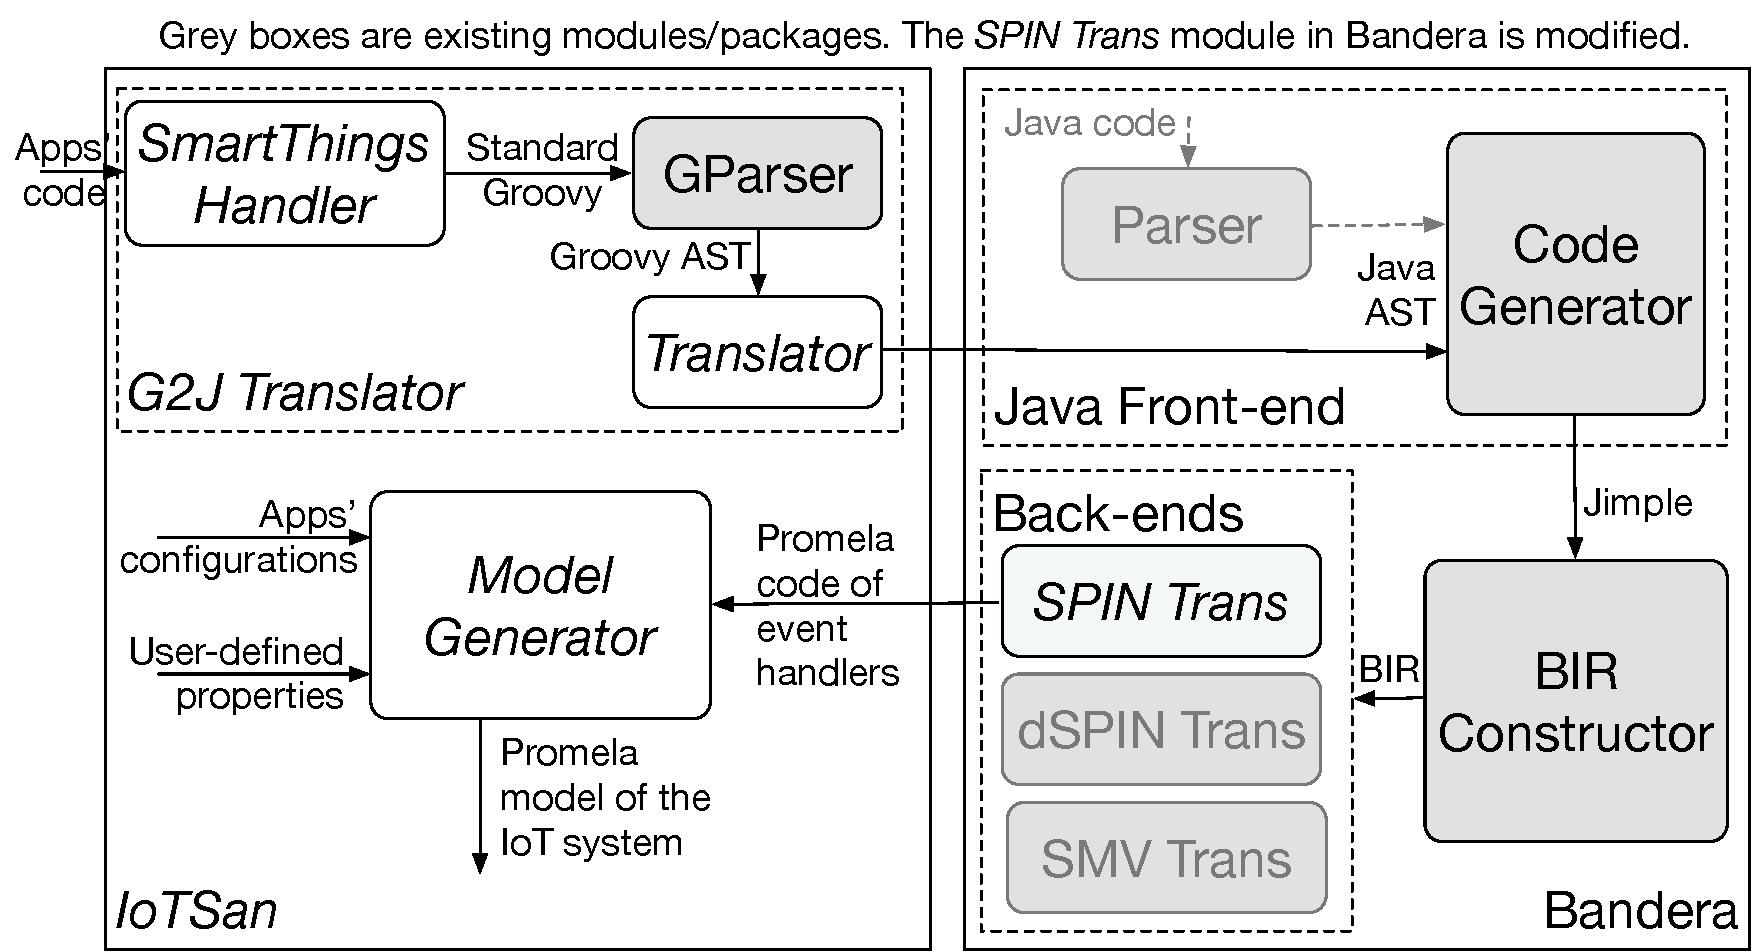
\includegraphics[width=3.8in]{IoTSanBanderaRelation}
%\vspace{-0.3in}
\caption{\textcolor{black}{\sys is built around Bandera.}}
%: the package \textit{org.codehaus.groovy} is used for the module GParser and the \textit{SPIN Trans} moduel in Bandera is modified.
\label{IoTSanBanderaRelation}
\end{center}
%\vspace{-0.25in}
\end{figure}


The key component we develop is the G2J Translator (see Figure~\ref{IoTSanBanderaRelation}),
which translates the smart app Groovy source into Java's Abstract Syntax Trees (ASTs).
In addition, the \textit{SmartThings Handler} is designed to handle the new language syntaxes introduced by SmartThings,
and the \textit{GParser} parses the regular Groovy source code into Groovy ASTs.
Basically, each smart app in Groovy is translated into a Java class,
whose method comprises of a method's header and a block of statements.
The translation procedure of a block is straightforward:
iterate through the statement list of the input Groovy block,
translate each Groovy statement into Java,
add the result to a list of Java statements,
and build a Java block from the result list.
To implement these,
we extended the Groovy compiler (\emph{org.codehaus.\allowbreak groovy})
which is then integrated into the Bandera's front-end.
%Below we describe how we address the above challenges.
%The translation procedure consists of two phases viz., (i) handling SmartThings' built-in utilities and (ii) translating Groovy's AST into Java's AST. Let us discuss this procedure in detail in the nutshell.

\section{Handling SmartThings' Language Features}
%Since SmartThings does not open the source code of its compiler, we build a library of SmartThings' platform based on their documentation \cite{Samsung:smartthingsapi}.
%Each object (\textit{e.g.}, attribute, command, capability, state, event, and device) is modeled by a Groovy class. All of these classes are packaged into a library, which is automatically imported by \textit{GParser} when parsing apps' source files.
There are several new language syntaxes introduced in SmartThings.
%examples of which are in Figure~\ref{inputexample}.
Our \textit{SmartThings Handler} parses these new syntaxes and converts them into
vanilla Groovy code using specifications based on the domain knowledge of SmartThings.
For instance, (as can be seen in {\color{black}in Figure~\ref{inputexample}) each $input$ function} defines a global variable (or a class field) of the app.
Therefore, we traverse the Groovy's AST of the app and visit all $input$ functions to extract all global variables of the app.
%$input$ method of SmartThings to get configuration information from users. Let us consider an example of an $input$ use case: \textit{input(name: ``color", type: ``enum", title: ``Color", options: [``Red",``Green",``Blue",``Yellow"])}, where $name$ defines the name of the variable that will be created in this smart app to reference this input; $type$ can be $capability.capabilityName$, $bool$, $decimal$, $email$, $enum$, $time$, $text$, $phone$, and so on; $option$ is a list of all possible values for this input.
In addition, apps can use some predefined objects or variables (\eg, $location$) and APIs (\eg, $setLocationMode$),
which are not defined in vanilla Groovy. Therefore, we manually add definitions of these global objects.
%Regarding their method definitions, we leave them as empty during the translation phase (so that the code compiles),
%but populate them during the modeling phase (see \S\ref{sec:model}).
%remove some SmartThings' built-in utilities (\textit{e.g.}, definition and preferences), which are not understandable by standard Groovy Compiler.

%\zhiyun{I'm not clear what we are doing here. After we extract the global variables from input, what do we do? Do we convert them into explicit variable definitions in Promela?}

%Moreover, an app can use some predefined variables, \textit{e.g.}, $location$, and APIs, \textit{e.g.}, $setLocationMode$. Then, we explicitly add definitions of the global variables as class fields and common APIs as local methods to the class of the app.

%: extract global variables used in the source file, and add definitions of these global variables and common SmartThings' objects (\textit{e.g.}, \textit{location} and APIs) to the source file;

%SmartThings allows apps to register callback functions (\textit{i.e.}, event handlers) - entry points of apps - for interested events via the $subscribe$ method. Since we need the info of event handlers in analyzing app dependency and generating Promela model, we also extract this info in this phase. Similar to the $input$ extraction, we also traverse the Groovy's AST of an app and visit all $subscribe$ method calls to get the subscribing info. \zhiyun{I understand that it is where you implement the callback function analysis, but this does not look like the translator's job. Can you check if this has anything to do with translation? The only thing I can image is that we may need to simulate the callback function ourselves because again the source code of the SmartThings framework is not available. However, logically I'd consider this more related to the modeling of the SmartThings system instead of part of the translator.}

\begin{figure}[tb]
	\ssp
    \centering
    %\raggedright
    \begin{subfigure}[t]{2.7in}
        \centering
        %\raggedleft
        %\includegraphics[width=1.3in]{groovycode}
		\lstinputlisting[language=groovy]{./code/groovycode.groovy}
		%\vspace{-0.12in}
        \caption{Groovy's code}
        \label{groovycode}
    \end{subfigure}\\
    %\vspace{-0.05in}
    \begin{subfigure}[t]{4.35in}
        \centering
        %\raggedleft
        %\includegraphics[width=2.4in]{javacode}
		\lstinputlisting[language=groovy]{./code/javacode.java}
				%\vspace{-0.12in}
        \caption{Corresponding Java's code}
        \label{javacode}
    \end{subfigure}
%\vspace{-0.1in}
    \caption{Example of translating a Groovy method into the corresponding Java's method.}
    \label{translationexample}
%\vspace{-0.22in}
\end{figure}

\section{Type Inference}
%{\color{red} We may use Gradual Typing with Unification-based Inference.}
%As mentioned above, Promela requires static typing of every declared variable, and therefore we need to perform type inference on Groovy code.
%\textit{org.codehaus.groovy}
Although the Groovy Compiler \textit{org.codehaus. groovy} already has a sub-package \textit{CompileStatic} for performing static type inference,
it only works when the argument type and the return type of a method are given.
In other words, a variable declared inside a method can take different runtime types depending on the argument type.
Thus, we still need to infer the argument and return type statically.
To do so, we consult the calling context of each method invocation
by recursively tracking the arguments and return values to their corresponding
anchor points---declaration of variables with explicit types (Groovy supports static typing as well),
assignment to constant values
(\eg, we can infer that the type of variable $a$ is numeric from \textit{def a = 0}),
assignment to return values of known APIs, and known objects and their properties.
The inference procedure works roughly as follows.
When traversing the AST of a method, we store the names and data types of variables at anchor points;
the types of other variables are inferred by propagating the types from anchor points.
This is done iteratively until we find no more new variables whose type can be inferred.


\section{Handling Groovy's Built-in Utilities}
%Another challenge is that since we are translating Groovy into Java which is then fed to Bandera.
Another challenge arises when we translate Groovy into Java for use with Bandera.
We find that Bandera understands only a very basic set of Java.
For instance, it supports only the $array$ type natively.
In contrast, Groovy's collection types (\eg, $Collection$, $List$, $ArrayList$, $Set$, $Map$, and $HashSet$)
all need to be translated into Java's $array$ type.
We support the popular collection types that are commonly used in smart apps.
An example is shown in Figure~\ref{translationexample} that translates one Groovy list into a corresponding Java implementation using array.
Since the type of \textit{switches} and \textit{onSwitches} is \textit{List of STSwtich},
we infer the return type of \textit{onSwitches()} method as \textit{List of STSwtich},
which is translated into Java's array type (\ie, \textit{STSwitch[]}).
The $+$ operation on \textit{List} type (line 2 in Figure~\ref{groovycode}) is
\textcolor{black}{automatically} translated into corresponding Java's code
(lines 2-17 in Figure~\ref{javacode}).
Finally, since this method is a non-void method,
we add an explicit $return$ statement (line 18 in Figure \ref{javacode}).






%\vspace{-0.13in}
\chapter{Configuration Extractor}
\label{sec:extractor}

IoT platforms typically provide a mobile companion app and/or a web-based app
to manage and configure smart apps and devices.
For Samsung SmartThings, we develop a crawler in Java,
using the \href{https://jsoup.org/}{\textit{Jsoup}} package to automatically extract the system's
configuration from the management web app~\cite{Samsung:smartthingsmanage}.
Given a SmartThings account (user's name and password),
the crawler logs in to the management web app
and extracts (i) installed devices, (ii) installed smart apps, and
(iii) configurations of apps.
%We also provide users with an interface to select the list of safety properties (more details in \S~\ref{sec:desiredproperty}) they need verified. 
Moreover, whenever a user installs a new generic smart device (\eg, a smart power outlet),
we have an interface to get the device association info (\eg, this new outlet is used to control an AC) from the user.
The extracted configuration is then saved to a file and used later by the \textit{Model Generator}.
The process is straightforward and we omit the details in the interest of space.

%\vspace{-0.15in}
\chapter{Model Generator}
\label{sec:model}

\section{Modeling an IoT system}
To correctly verify safety properties, we need to model two key components (not part of the app code):
(i) the IoT platform and its interactions with smart apps and
(ii) IoT devices and their interactions with smart apps.
{\color{black}IoT platforms~\cite{iftttpage,Samsung:smartthings,Apple:homekit,Amazon:alexa,Microsoft:iot} typically provide apps with some methods to register callback functions (\ie, event handlers).
Based on apps' configurations provided by the \textit{Configuration Extractor}, we model these special registration functions so as to invoke callbacks at appropriate times.}
\begin{comment}
With regards to the SmartThings platform, we first need to model its platform SDKs, which are unfortunately not open sourced.
Thus, we model the major classes and methods based on the SmartThings documentation~\cite{Samsung:smartthingsapi}.
The example classes include \textit{Command, Attribute, Event, Mode, State, and Location.}
%Each object (\textit{e.g.}, attribute, command, capability, state, event, and device) is modeled by a Groovy class.
%All of these classes are packaged into a library, which is automatically imported by \textit{GParser} when parsing smart apps' source files. \zhiyun{I think this is more related to modeling of the SmartThings framework and not so much about translator (so I moved it here)}
In addition, the SmartThings platform allows apps to register callback functions (\ie, event handlers)
via $subscribe$ and $schedule$ methods.
%Since we need the info of event handlers in analyzing app dependency and generating Promela model, we also extract this info in this phase.
We model these special registration functions so as to invoke callbacks at appropriate times.
\end{comment}


We model IoT devices (sensors and actuators) as per their specifications.
Note that both sensors and actuators can generate events of interest to apps.
For instance, a motion sensor can generate motion active/inactive events
whereas a door lock (actuator) can generate status update events (locked\allowbreak /unlocked).
%The difference is that actuators can take commands from apps (\eg, lock/unlock a door).
Each device is modeled as having an event queue
and a set of notifiers to inform the smart apps that have subscribed to specific types of events.
Currently, we support 30 different IoT devices.
%We use a global array to store all devices of same type in a system (\textit{e.g.}, $\_g\_STSwitchArr$ stores info of all switch devices in a system).
%A device assigns a specific slot in its subscriber notifiers to each subscriber. Whenever an event happens, a device will update its subscriber notifiers. A smart app will check its assigned slot in the subscriber notifiers of its subscribed device to see if any event happens. If the assigned slot is greater than $0$, the smart app will check the event queue to get the latest events, process them, and reset the slot to $0$. A smart app may send commands to some actuators via method call.
{\color{black} Note here that we model events generated by
the environment (\eg, $sunrise$ and $sunset$) as sensor generated inputs
and location mode changes 
(\textit{e.g.}, $Home$, $Away$, and $Night$) as actuations;
thus inputs such as users leaving home (sensed input) can trigger the mode to change from $Home$ to $Away$ (actuation).} 

{\color{black}We model system time as a monotonically
increasing variable. We extract the triggering times and callback functions from the scheduling
method calls. The callback functions are then triggered at appropriate times based on the value of
the modeled system time.}

\begin{comment}
{\color{black} Note here that we model the environment event (\eg, $sunrise$ and $sunset$) manager as a sensor device
and location mode 
(\textit{e.g.}, $Home$, $Away$, and $Night$) manager as an actuator,
which can take commands from some apps such as users leaving home and may trigger the mode to change from \textit{Home} to \textit{Away}.}
\end{comment}

Algorithm~\ref{alg:smarthingprocess} shows the pseudo code of the main process that models behaviors of an IoT system.
%\zhiyun{What is the ``SmartThings process''? It is the overall event simulation loop of the whole IoT system? Can we simplify the pseudo code? It is too long at the moment} \thomas{Yeah, it is the event simulation loop of the whole IoT system. I have simplified it. What do you think?}.
The model checker enumerates all possible permutations of the input physical events
up to a maximum number of events per user's configuration
to exhaustively verify the system.
At each iteration, a sensor and a corresponding physical event in the permutation space are selected (line 2).
Then, the selected sensor updates its state and event queue,
and notifies its subscribers of the state change event (line 3).
When an event is pending,
it is dispatched to the subscribed apps and the corresponding event handlers of apps are invoked to handle the event (lines 4-6).
Each event handler may send some commands to some actuators,
which may generate some new cyber events and trigger event handlers of the subscribers.

\begin{algorithm}[tb]
%\small
\ssp
\small
 \caption{Modeling an IoT system}
 \label{alg:smarthingprocess}
 \begin{algorithmic}[1]
 %\renewcommand{\algorithmicrequire}{\textbf{Input:}}
 %\renewcommand{\algorithmicensure}{\textbf{Output:}}
 %\REQUIRE None
 %\ENSURE  None
  %\COMMENT{\textbf{Main event loop of an IoT system}}
  \FOR[\textit{Main event loop of an IoT system}]{$i = 1$ to maximum number of events}
  \STATE Select a sensor and a corresponding event in the permutation space \COMMENT{\textit{Generate a physical event}}
  \STATE sensor\_state\_update(evt)
  \WHILE {any event pending}
  	\STATE dispatch\_event(evt) \COMMENT{\textit{Dispatch the pending event to the subscribed apps and invoke the corresponding app\_event\_handler(evt) to process the event}}
  \ENDWHILE
  \ENDFOR
  \\ \COMMENT{\textbf{sensor\_state\_update(evt)}}
  \IF {$evt \neq$ current state of the sensor}
 	\STATE Add the $evt$ to the event queue
 	\STATE Update the state of the sensor
 	\STATE Notify the subscribers of the state change event
 \ENDIF
  \\ \COMMENT{\textbf{app\_event\_handler(evt)}}
  \IF {some conditions hold}
 	\STATE Send some command to some actuator \COMMENT{\textit{Invoke actuator\_state\_update(evt), which may subsequently generate some new event}}
 \ENDIF
  \\ \COMMENT{\textbf{actuator\_state\_update(evt)}}
  \STATE Verify conflicting and repeated commands violations
  \IF {$evt \neq$ current state of the actuator}
 	\STATE Add the $evt$ to the event queue
 	\STATE Update the state of the actuator
 	\STATE Notify the subscribers of the state change event
 \ENDIF
 \end{algorithmic}
 \end{algorithm}



To model natural or induced (\textit{e.g.}, using jamming~\cite{5473884}) device/communication 
failures, 
when generating a sensor event we enumerate two scenarios:
(i) the sensor is available/online and (ii) the sensor is unavailable/offline.
Similarly, whenever receiving a command from a smart app,
an actuator may be either online or offline.
If a device is offline, it will not change its state and hence {\em not} broadcast a state change event to its subscribers. {\color{black}If a device is online, 
the communication (\ie, sending a state change event or receiving a command) between the device and the hub/cloud may either succeed or fail (we enumerate both cases).}

\begin{table}[tb]
\ssp
%\vspace{-0.16in}
\caption{Sample safe physical states.}
%\vspace{-0.12in}
\label{table:racescenarios}
\centering
{
{\color{black}\begin{tabular}{| p{1.9cm} | p{0.5cm} | p{11.5cm} |}
\hline
\bf Category & \bf \# & \bf Property\\
\hline
\multirow{5}{1.9cm}{Thermostat, AC, and Heater} & 1 & Temperature should be within a predefined range when people are at home\\ \cline{2-3}
 & 2 & An AC and a heater should not be both turned on\\ \cline{2-3}
 & 3 & The cooling set-point of a thermostat should be set to a value which is the same as the configured one\\ \cline{2-3}
 & 4 & The heating set-point of a thermostat should be set to a value which is the same as the configured one\\ \cline{2-3}
 & 5 & Thermostat should be turned off when a window/door is opened\\ \cline{2-3}
\hline
\multirow{8}{1.9cm}{Lock and door control} & 1 & The main door should be locked when no one is at home\\ \cline{2-3}
& 2 & The main door should be locked when people are sleeping\\ \cline{2-3}
& 3 & The main door should be locked when no one is at home and smoke detector state is clear\\ \cline{2-3}
& 4 & The main door lock should be locked when people are sleeping and smoke detector state is clear\\ \cline{2-3}
& 5 & A door control should be closed when no one is at home\\ \cline{2-3}
& 6 & When a door is closed, a lock should be locked\\ \cline{2-3}
& 7 & When all people leave home, some locks should be locked and location mode should be changed to Away\\ \cline{2-3}
& 8 & A door should be locked after being unlocked\\ \cline{2-3}
\hline
\multirow{3}{1.9cm}{Location mode} & 1 & Location mode should be changed to Away when no one is at home\\ \cline{2-3}
 & 2 & Location mode should be changed to Home when some one arrives at home\\ \cline{2-3}
 & 3 & Location mode should be set to the configured mode at sunset\\ \cline{2-3}
\hline
\multirow{3}{1.9cm}{Water and sprinkler} & 1 & Soil moisture should be within a predefined range\\ \cline{2-3}
& 2 & A water valve should be closed when a water sensor's state is wet\\ \cline{2-3}
& 3 & When there is water leakage, an SMS/Push message should be sent to the owner\\ \cline{2-3}
\hline
\multirow{5}{1.9cm}{Others} & 1 & Some devices should not be turned on when no one is at home\\ \cline{2-3}
& 2 & A tone should not beep when people are sleeping\\ \cline{2-3}
& 3 & A fridge should be always on\\ \cline{2-3}
& 4 & A music player should not play when people are sleeping\\ \cline{2-3}
& 5 & An audio notification should not play when people are sleeping\\ \cline{2-3}
\hline
\end{tabular}}
}
%\vspace{-0.17in}
\end{table}

\begin{table}[tb]
\ssp
%\vspace{-0.16in}
\caption{Sample safe physical states (continue).}
%\vspace{-0.12in}
\label{table:racescenarios1}
\centering
{
{\color{black}\begin{tabular}{| p{1.9cm} | p{0.5cm} | p{11.5cm} |}
\hline
\bf Category & \bf \# & \bf Property\\
\hline
\multirow{14}{1.9cm}{Security and alarming} & 1 & An alarm should not strobe/siren when smoke detector state is clear\\ \cline{2-3}
& 2 & A surveillance camera should be always on\\ \cline{2-3}
& 3 & Bulbs around surveillance cameras should be on when it is dark\\ \cline{2-3}
& 4 & An alarm should strobe/siren when detecting smoke\\ \cline{2-3}
& 5 & An alarm should strobe/siren when a lock is unlocked and people are sleeping or not at home\\ \cline{2-3}
& 6 & An alarm should strobe/siren when detecting motion and people are sleeping or not at home\\ \cline{2-3}
& 7 & An audio notification should play when detecting motion and no one is at home\\ \cline{2-3}
& 8 & Notification should be sent when a door is opened and no one is at home\\ \cline{2-3}
& 9 & When there is smoke, an SMS/Push message should be sent to the owner\\ \cline{2-3}
& 10 & When there is motion and no one is at home, an SMS/Push message should be sent to the owner\\ \cline{2-3}
& 11 & Alarm mode should be enabled when location mode changes to target mode\\ \cline{2-3}
& 12 & Alarm mode should be enabled when all people leave home\\ \cline{2-3}
& 13 & A water valve should be opened when detecting smoke\\ \cline{2-3}
& 14 & An alarm should be triggered when a door is opened\\ \cline{2-3}
\hline
\end{tabular}}
}
%\vspace{-0.17in}
\end{table}

\section{Concurrency Model}
{\color{black}Since an app's event handler is only triggered by the subscribed event(s) and event handlers of different apps do not share any global variable~\cite{iftttpage,Samsung:smartthings,Apple:homekit,Amazon:alexa,Microsoft:iot}, the execution of an app's event handler can be considered as atomic. 
This means that the concurrency level of a model only depends on the interleaving of apps' event handlers. To model a concurrent IoT system therefore, we 
only need to verify the behaviors of the system with interleavings of all of 
the external events (\eg, smoke detected) sensed by sensors and internal events (\eg, unlocked) caused by apps' behaviors. Even though the events are concurrent, the interleaving is in fact reflected by the order of the (incoming) events processed by event handlers, \ie, we can obtain the strict concurrency by 
considering all order permutations of  external and internal events. 
However, this approach takes a very long verification time 
as the number of events grow, and causes the state space to explode. Instead, we can obtain a weaker concurrency by considering the permutations of only external events in a sequential design shown in Algorithm ~\ref{alg:smarthingprocess}. This implicitly assumes that the internal events associated with
an external event are handled atomically in order.
It is unclear if enforcing strict concurrency would lead to 
the discovery of more unsafe states. We experiment with the two design options with several small systems and find that the sequential approach offering
weak consistency, discovered all violations that the strict concurrent model found. Based on this, we use the sequential approach given that it 
significantly mitigates the time complexity of execution.}


\section{The IoT System Model in Promela}
{\color{black}With the concurrent approach, each device and smart app is modeled by a process (\ie, \textit{proctype}).
There is also a process for generating the sensed and environmental events.
The processes communicate with each other using message passing (\ie, \textit{chan}).
We use a single process for the whole system with our sequential design,
using \textit{inline} methods to model the behavior of devices and smart apps.
The devices, smart apps, and event generators, communicate via shared global variables.}


%\zhiyun{need to mention the external event vs. internal event}\thomas{In the Overview section, we have briefly explain this in the chain action of events: external event = physical event and internal event = event in cyber}




%\subsection{Verification of \textcolor{black}{User-defined Properties}}\label{sec:desiredproperty}
\section{Safety Properties}
We seek to verify \textcolor{black}{45 properties of the following types}:
%\zhiyun{need to tell how many properties we check in total either here or in the evaluation section}
\begin{itemize}
\item {\em Free of conflicting commands} {\color{black}\cite{Newcomb:2017:ICI:3133850.3133860}}: When a single external event happens,
an actuator {\color{black}should not receive} two conflicting commands (\eg, both on and off) -- (1 property).

\item {\em {\color{black} Free of} repeated commands}: When a single event happens,
an actuator {\color{black}should not receive multiple repeated commands of the same type or with the same payload -- (1 property).
The latter could indicate a potential DoS or replay attack.

%{\color{black}The first two classes of properties can be asserted easily (line 16 in Algorithm~\ref{alg:smarthingprocess}).}}
}

\item {\em {\color{black}Safe} physical states}:
Table~\ref{table:racescenarios} and Table~\ref{table:racescenarios1} show some sample {\color{black}safe physical} states that the user desires the system to satisfy.
These kinds of properties can be verified using linear temporal logic (LTL)~\cite{Baier:modelchecking}
-- (38 properties).
We envision that a more complete list will likely be provided by safety regulations associated with the IoT industry in the future.

\item {\em {\color{black} Free of} other known suspicious app behaviors---security-sensitive command and information leakage}:
Examples of security-sensitive commands are \textit{unsubscribe} (disabling an app's functionality) {\color{black} and creating fake events (\eg, an app may generate a ``smoke detected'' event when there is no smoke in the physical environment); we raise violations when such commands are executed.}
Information leakage can occur with \textit{sending SMS} and \textit{using network interfaces}.
When \textit{sending SMS} is triggered, for instance,
we check whether the recipient matches with the configured phone number to prevent leakage -- (4 properties).

\item {\em Robustness to device/communication failure}: An app should quickly check
that a command sent to an actuator was acted upon to be robust to device and communication
failures. Upon detecting a failure, the app should notify users via SMS/Push messages.
This property can be verified using LTL as well -- (1 property).
\end{itemize}

Note that we provide users with an interface to select the list of safety properties they want to verify. \textcolor{black}{Based on the device association information (recall \S~\ref{sec:extractor}) provided by the \textit{Configuration Extractor}, the LTL format of the selected properties are automatically generated.}

\section{Example} Consider the smart home of a single owner Alice (say),
which comprises of a smart lock that controls the main door viz., \texttt{Door Lock},
and a presence sensor viz., \texttt{Alice's Presence}
(which checks if Alice is at home).
Assume that Alice installs two smart apps: \textit{Auto Mode Change},
which manages the location mode based on the events from \texttt{
Alice's Presence}
and, \textit{Unlock Door}, which unlocks the \texttt{Door Lock} based on explicit user input
or a ``location mode'' change event.
When this system is analyzed by the model checker, a violation is detected as described below.

\hfill \break

\begin{figure}[tb]
\ssp
\begin{center}
    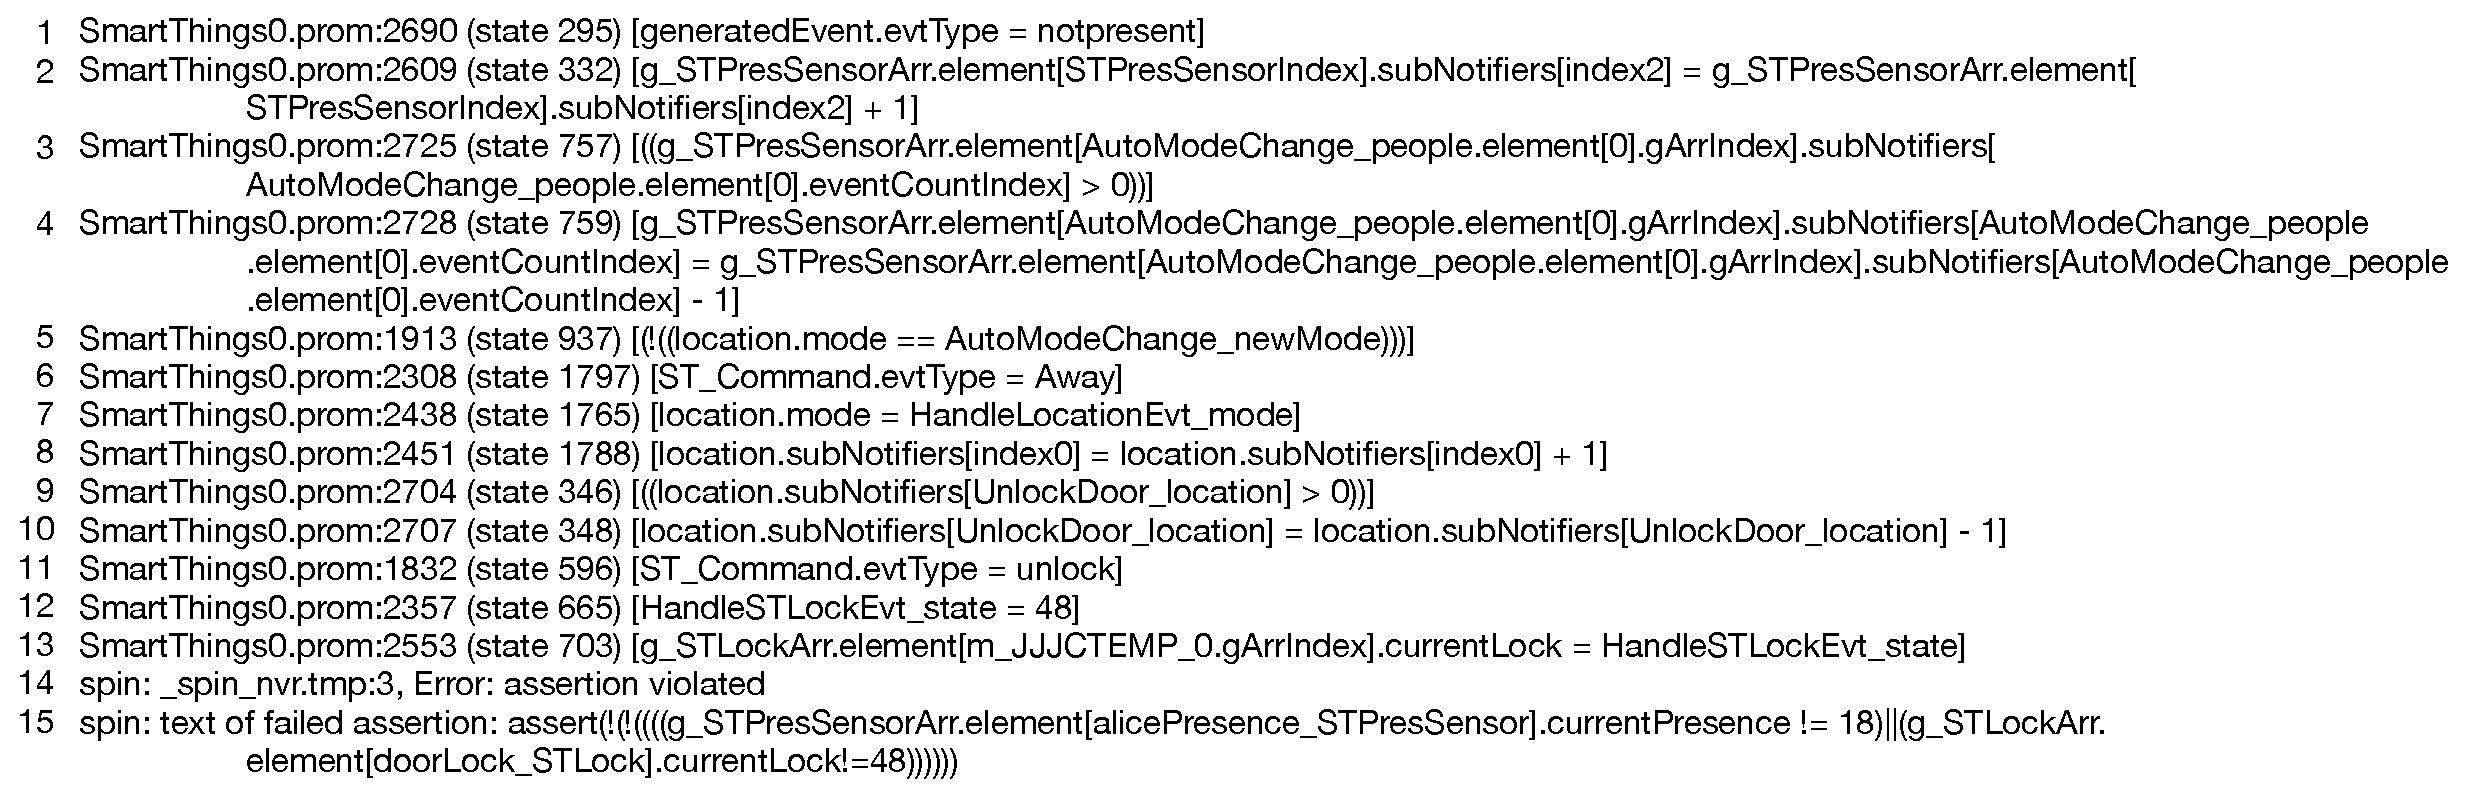
\includegraphics[width=6.1in]{verificationlog}
	%\mbox{\lstinputlisting[language=groovy]{./code/violationlog.cc}}
	%\parbox[6.0in]{\lstinputlisting[language=groovy]{./code/violationlog.cc}}
	%\lstinputlisting[language=groovy]{./code/violationlog.cc}
	%\vspace{-0.17in}
    \caption{Example violation log (filtered).}
	\label{verificationlog}
\end{center}
%\vspace{-0.2in}
\end{figure}


Figure~\ref{verificationlog} shows the (filtered) violation log (a counter-example) output by \spin.
The format of each line in the violation log is as follows:
file name (\textit{SmartThings0.prom}), line number, state number, and the executed code.
In particular, the counter example has the following steps.
{\bf (1)} The event \textit{not present} is generated by \texttt{Alice's presence} if Alice leaves home (line 1)
and its subscribers are notified of this state change (line 2).
{\bf (2)} The app \textit{Auto Mode Change} reads and processes this state change event (lines 3-5)
and notifies the location manager to change the location mode to \textit{Away} (line 6).
{\bf (3)} The location manager changes its mode and notifies its subscribers of this change (lines 7-8).
{\bf (4)} The app \textit{Unlock Door} reads and processes this mode change event (lines 9-10)
and sends an $unlock$ command to the device \texttt{Door Lock} (line 11),
which unlocks the door (lines 12-13).
Thus, the system enters an unsafe physical state (\ie, the main door is unlocked when no one is at home) (lines 14-15).

Upon closer inspection, the description of \textit{Unlock Door} suggests
that it unlocks the door {\em only upon user input}.
However, in practice, it also unlocks the door whenever the location mode changes
(\ie, there is an inconsistency between the app's description and its implementation).

%\vspace{-0.15in}
\chapter{Output Analyzer}
\label{outputanalyzer}

%The cause of a violation can be either bad configuration or bad app.
The \textit{Output Analyzer} {\em attributes} a violation to either a misconfiguration or a malicious app
using a heuristic-based algorithm.
The algorithm consists of two phases.
In the first phase, when a user installs a new smart app,
the output analyzer enumerates all possible configurations for this app.
It verifies if the user-defined properties hold with each configuration independently.
If the proportion of violations (violation ratio) is greater than a predefined threshold (\eg, 90\%),
the new smart app is attributed as a malicious app.

If this is not the case, in the second phase, the new app is verified
in conjunction with other apps that were previously installed by the user.
Again, all configurations are considered.
If the violation ratio is greater than a predefined threshold,
the new app is attributed as a bad app and a report is provided to the user.
Otherwise, the violation is attributed to misconfiguration and
suggestions of safe configurations with regards to the user defined properties
are provided.
If there is no violation, a successful verification is reported.
%Based on the report of our system, the user can decide to either remove the new app or change its configuration if any violation is detected.

%\textbf{Example of calculating all possible configurations for an app}: Let us consider the app \textit{Auto Mode Change}, which requires a user to configure a list of presence sensors. Assume that there are three presence sensors in the IoT system: \textit{dadPresence}, \textit{momPresence}, and \textit{sonPresence}. There will be seven possible configurations for this app: (\textit{dadPresence}), (\textit{momPresence}), (\textit{sonPresence}), (\textit{dadPresence}, \textit{momPresence}), (\textit{dadPresence}, \textit{sonPresence}), (\textit{momPresence}, \textit{sonPresence}), and (\textit{dadPresence}, \textit{momPresence}, \textit{sonPresence}). If an app has several inputs, the possible configurations will be all possible combination of the inputs.

%\vspace{-0.12in}
\chapter{Evaluations}
\label{sec:eval}
%The implementation of \sys was implicitly described in prior sections.
%(most modules
%were implemented in Java).
Our experiments (model checking) are performed on a MacBook Pro with macOS Sierra, 2.9 GHz Intel Core i5, 16 GB 1867 MHz DDR3, and 256 GB SSD.
We check if there are violations of the properties 
discussed in \S\ref{sec:model}.
%Table~\ref{table:racescenarios}
We also look at other performance metrics such as the running times,
and the scale ratio (which quantifies the reduction in the number of event handlers
to be jointly verified) to evaluate \sys.

%\vspace{-0.17in}
\section{Test Cases and Configurations}
We perform four different sets of experiments described below.
The first three examine the fidelity with which bad apps and configurations are identified.
The last set evaluates the performance of different design choices we make.

{\bf Market apps with expert configurations:}
We check the safety properties with
150 apps (assuming they are benign) from the {\color{black}SmartThings' market place \cite{SmartThingsGitHub,STCommunitySmartApps,Samsung:smartthingsmanage}.}
We (the authors) came up with independent
configurations for the apps (based on common sense with regards to how the apps may be used).
To illustrate, consider the app \textsl{Virtual Thermostat}, the required input to which is shown in Figure~\ref{inputexample}.
Assume that the following devices are deployed:
(1) one temperature sensor (myTempMeas), (2) one outlet to control the heater (myHeaterOutlet),
(3) one outlet to control the air conditioner (myACOutlet),
(4) one outlet to control the light in the living room (livRoomBulbOutlet),
(5) one outlet to control the light in the bedroom (bedRoomBulbOutlet),
(6) one outlet to control the light in the bathroom (batRoomBulbOutlet),
(7) one motion sensor in the living room (livRoomMotion),
and (8) one motion sensor in the bathroom (batRoomMotion).
Our configuration is as follows:
myTempMeas for the temperature sensor (line 3 in Figure~\ref{inputexample}),
myACOutlet for ``outlets" (line 7 in Figure~\ref{inputexample}),
$75$ as the ``{\color{black} setpoint}" temperature if people are present (line 9 in Figure~\ref{inputexample}),
livRoomMotion for ``motion" (line 12 in Figure \ref{inputexample}),
$10$ ``minutes" for turning off the AC/heater when no motion is sensed (line 15 in Figure~\ref{inputexample}),
%\krish{Say what this does as in prior cases},
$85$ as the ``emergencySetPoint" temperature at which the AC is turned on (to set) regardless of
whether people are present (line 18 in Figure \ref{inputexample}),
and ``cool" for ``mode" (line 21 in Figure \ref{inputexample}).
%\krish{Unless something isn't obvious above no need for this. But provide some description as the ones I did}
%We think that this configuration is reasonable because those of both air conditioner and heater, (2) ``cool" instead of ``heat" should go with air conditioner, and (3) other remaining fields are quite straightforward.

We randomly divide the 150 apps into six groups (25 apps per group) with one configuration each,
and feed them into \sys.
Upon encountering a violation, we remove the minimum number of the associated apps (\textit{e.g.}, if there are two apps causing conflicting commands, we randomly remove one of them);
%\krish{what are conflicting commands ? Hopefully this has been described earlier.}\thomas{Yes, it is}
we then iterate the process. The experiment stops when no violation is detected.
These experiments are performed with and without device/communication failures.

\hfill \break

{\bf Market apps with non-expert configurations:}
To eliminate biases, we also conduct a user study where we request 7 independent student volunteers
to configure 10 groups of apps with the assumption that they would deploy them at home.
Each group comprises of about 5 related apps (as determined by our app dependency analyzer).
A group receives one configuration from each volunteer and this leads to a total of 70 configurations.
Our Office of Research Integrity determined that
there was no need to go through an IRB approval process (since no private information is collected).

{\bf Malicious apps:}
We consider 25 malicious apps created in~\cite{Jia:contexiot}.
In this set, we find that only 9 apps are relevant
to our evaluations (\textit{e.g.}, affect the physical state and can be compiled correctly by the SmartThings' own web-based IDE).
%\textcolor{black}{among 25 apps, since there are several duplicates, we have 20 apps after removing the duplicates; moreover, four apps (\textit{i.e.}, \textit{BackDoorPincodeInjection}, \textit{LockAccessRevocation}, \textit{LockManager}, and \textit{MaliciousCameraIPC}) get compile errors with Samsung SmartThings' web-based IDE (16 apps remaining); we manually analyzed the source code of the app \textit{Disabling Vacation Mode} and did not find any malicious behaviors (15 apps remaining); attacking techniques done by the two apps \textit{CO Detector} and \textit{Hello Home} are out of our problem scope because they just add some extra content to an SMS message (13 apps remaining);
There are four apps that \sys cannot currently handle viz., \textit{Midnight Camera}, \textit{Auto Camera}, \textit{Auto Camera 2}, and \textit{Alarm Manager}, since they dynamically discover and control the devices in the system; we will extend \sys to handle such apps in future work.
%however, their malicious functions can be detected by \sys; for example, the three apps (\textit{Auto Camera}, \textit{Auto Camera 2}, and \textit{Alarm Manager}) would violate information leakage property when the command \textit{httpPost} is executed, and the app \textit{Midnight Camera} would violate the property \textit{A specific light close to surveillance camera is turned off at night}. \zhiyun{I don't understand why we can detect problems with three of these apps even when we admit \sys cannot handle them.}\thomas{These apps cannot be modeled and verified by \sys. If we remove the ``dynamic discovery" code, these apps can be verified by \sys and their adversary techniques can be detected by \sys using the properties we have defined.}
%\thomas{Do we need to explain why other apps are not relevant here?} . \krish{Yes -- this is where you would discuss that.}
We evaluate whether \sys correctly attributes these malicious apps when they are installed together with other apps.
The configurations of the 9 malicious apps are identical to those
in \cite{Jia:contexiot}. We also choose 11 potentially bad apps (found via the previous experiments) from the market place 
for a total of 20 bad apps. In conjunction, we select 10 good apps from the market place to create a reasonable input set. Here, we specifically evaluate the fidelity of our attribution module. %with the input data set and the stable system.

\begin{table*}[tb]
\scriptsize
\caption{Verification results with market apps.}
%\vspace{-0.12in}
\label{market_apps}
\centering
%\bf
{\begin{tabular}{| p{2.2cm} | p{1.4cm} | p{4.5cm} | p{4.5cm} |}
\hline
{\bf Violation type} & {\bf Number of violations} & {\bf Example violated property} & {\bf Apps related to example}\\
\hline
Conflicting commands & 8 & A light receives ``on" and ``off" simultaneously & (Brighten Dark Places, Let There Be Dark)\\
%\hline
%2 & A configured outlet is turned off when someone is still at home & 1 & (Curling Iron)\\
\hline
Repeated commands & 10 & A light receives repeated ``on'' commands & (Automated light, Brighten My Path)\\
\hline
\multirow{2}{2.2cm}{Unsafe physical states} & \multirow{2}{*}{20} & A heater is turned off at night when temperature is below a predefined threshold & (Energy Saver)\\ \cline{3-4}
 & & The main door is unlocked when people are sleeping at night & (Light Follows Me, Light Off When Close, GoodNight, Unlock Door)\\ \cline{3-4}
\hline
\end{tabular}}
%\vspace{-0.12in}
\end{table*}

\begin{table}[tb]
\ssp
\scriptsize
\caption{Verification result with market apps, with volunteer configuration.}
%\zhiyun{violation ratio in this table and the violation ratio in the next table are both called the same thing but they are actually trying to capture different things. I think we should call it something else. Maybe ``Percentage of bad configurations''?} \thomas{I have modified the term.}
\label{user_market_apps}
\centering
{
\begin{tabular}{| c | p{5.5cm} | p{4.5cm} | p{2.0cm} |}
\hline
{\bf Group} & {\bf Violations} & {\bf Related Apps} & {\bf Percentage of bad configs}\\
\hline
\multirow{12}{*}{1}  & A microwave is turned on when no one is at home & Big Turn On, Auto Mode Change & 28.6\%\\ \cline{2-4}
	& \multirow{2}{5.5cm}{An AC and a heater are both turned on} & Big Turn On, Auto Mode Change & 28.6\%\\ \cline{3-4}
	&	& The Big Switch & 42.9\%\\ \cline{2-4}
	& \multirow{4}{5.5cm}{A heater is turned on when temperature is above a predefined threshold and no one is at home} & Big Turn On, Auto Mode Change & 28.6\%\\ \cline{3-4}
	&	& The Big Switch & 42.9\% \\[3ex] \cline{2-4}
	& \multirow{3}{5.5cm}{An AC is turned on when temperature is below a predefined threshold} & Big Turn On, Auto Mode Change & 42.9\%\\ \cline{3-4}
	&	& The Big Switch & 71.4\%\\
\hline
\multirow{13}{*}{2}  &  \multirow{9}{7cm}{Conflicting commands}  & Brighten Dark Places, Let There Be Dark! & 85.7\%\\ \cline{3-4}
	&	& Once a Day, Let There Be Dark! & 14.3\%\\ \cline{3-4}
	&	& Once a Day, Curling Iron & 71.4\%\\ \cline{3-4}
	&	& Once a Day, Light On Motion & 28.6\%\\ \cline{3-4}
	&	& Brighten Dark Places, Once a Day & 14.3\%\\ \cline{2-4}
	& \multirow{4}{5.5cm}{Repeated commands} & Curling Iron, Light On Motion & 42.9\%\\ \cline{3-4}
	&	& Once a Day, Let There Be Dark! & 14.3\%\\ \cline{2-4}
	& An AC and a heater are both turned on & Once a Day & 28.6\%\\ \cline{2-4}
	%&	& Light on Motion & 14.3\%\\ \cline{2-4}
	& A heater is turned on when temperature is above a predefined threshold & Once a Day & 28.6\%\\ \cline{2-4}
	%&	& Light on Motion & 14.3\%\\ \cline{2-4}
	& An AC is turned on when temperature is below a predefined threshold & Once a Day & 57.1\%\\ \cline{2-4}
	%&	& Light on Motion & 14.3\%\\
\hline
3 & No violation & & \\
\hline
\end{tabular}
}
\end{table}

\begin{table}[tb]
\ssp
\scriptsize
\caption{Verification result with market apps, with volunteer configuration (continue).}
%\zhiyun{violation ratio in this table and the violation ratio in the next table are both called the same thing but they are actually trying to capture different things. I think we should call it something else. Maybe ``Percentage of bad configurations''?} \thomas{I have modified the term.}
\label{user_market_apps1}
\centering
{
\begin{tabular}{| c | p{5.5cm} | p{4.5cm} | p{2.0cm} |}
\hline
{\bf Group} & {\bf Violations} & {\bf Related Apps} & {\bf Percentage of bad configs}\\
\hline
\multirow{9}{*}{4}  & An AC is turned off when temperature is above a predefined threshold & Energy Saver & 42.9\%\\ \cline{2-4}
	& 	A heater is turned off when temperature is below a predefined threshold & Energy Saver & 42.9\%\\ \cline{2-4}
	& \multirow{3}{5.5cm}{Repeated commands} & AND Switch, Away Mode With Eco Turn Off & 14.3\%\\ \cline{3-4}
	&	& AND Switch, Energy Saver & 14.3\%\\
\hline
5 & No violation & & \\
\hline
\multirow{8}{*}{6}  & \multirow{6}{5.5cm}{Repeated commands} & Automated light, Brighten My Path & 42.9\%\\ \cline{3-4}
	& 	& Automated light, Garage check open/close App & 14.3\%\\ \cline{3-4}
	& 	& Brighten My Path, Garage check open/close App & 14.3\%\\ \cline{2-4}
	%& An AC and a heater are both turned on & Brighten My Path & 28.6\%\\ \cline{2-4}
	%& An AC is turned on when temperature is below a predefined threshold & Brighten My Path & 28.6\%\\ \cline{2-4}
	& An AC is turned off when temperature is above a predefined threshold at night & Light Follows Me, Light Off When Close, Big Turn Off, Good Night & 14.3\%\\ \cline{2-4}
	%& A heater is turned on when temperature is above a predefined threshold & Brighten My Path & 28.6\%\\ \cline{2-4}
	& A heater is turned off when temperature is below a predefined threshold at night & Light Follows Me, Light Off When Close, Big Turn Off, Good Night & 14.3\%\\
\hline
7 & No violation & & \\
\hline
\multirow{4}{*}{8}  & Conflicting commands & Multi-way On/Off Toggle Switch Using a Modded PEQ Door Open/Close Sensor, Undead early warning & 57.1\%\\ \cline{2-4}
	& An AC and a heater are both turned on & Virtual Thermostat & 71.4\%\\ \cline{2-4}
	& An AC is turned on when temperature is below a predefined threshold & Virtual Thermostat & 42.9\%\\ \cline{2-4}
	& A heater is turned on when temperature is above a predefined threshold & Virtual Thermostat & 28.6\%\\
\hline
9 & No violation & & \\
\hline
10 & Repeated commands & Let There Be Light!, Delayed Command Execution & 28.6\%\\
\hline
\end{tabular}
}
\end{table}


\begin{comment}
{
{\em Fourth set of experiments:}
We evaluate the verification time against number of generated events with \sys. We use the apps in a specific group of apps which did not have any violations, from the user study.
%The group comprises of five apps and all of them belong to the same dependent set (\textit{i.e.}, the apps should be verified jointly).
Table \ref{verificationtimesetup} describes the devices used by the apps. We quantize the humidity measurement outputs to five values (\textit{i.e.}, 10\%, 30\%, 50\%, 70\%, and 100\% ) and the temperature measurement outputs to three values (\textit{i.e.}, 1, 2, and 3).
\begin{table}[!h]
\scriptsize
\caption{Experiment setup to evaluate verification time.}
\label{verificationtimesetup}
\centering
\begin{tabular}{| l | c | c |}
\hline
Device type & \# of devices & \# of states/device\\
\hline
Presence sensor & 3 & 2\\
\hline
Contact sensor & 1 & 2\\
\hline
Humidity measurement sensor & 1 & 5\\
\hline
Temperature measurement sensor & 1 & 3\\
\hline
Switch & 2 & 2\\
\hline
Lock & 2 & 2\\
\hline
\end{tabular}
\end{table}
}
\end{comment}

\textcolor{black}{{\bf Performance:}
We compare the performance of concurrent \textit{versus} sequential design.
We use two bad groups of apps viz., (Auto Mode Change, Unlock Door) and (Brighten Dark Places, Let There Be Dark),
and one good group of apps viz., (Good Night, It's Too Cold) that control 3 switch devices,
3 motion sensors, and 1 temperature measurement sensor.}

%\vspace{-0.1in}
\section{Identifying Unsafe Configurations}
%\section{ContexIoT's malicious apps}
%Among 25 malicious apps, since there are several duplicates, we have 20 apps after removing the duplicate ones. Moreover, four apps (\textit{i.e.}, \textit{BackDoorPincodeInjection}, \textit{LockAccessRevocation}, \textit{LockManager}, and \textit{MaliciousCameraIPC}) got compile errors with Samsung SmartThings' web-based IDE. Therefore, there are only 16 apps remaining. We manually configured the setting for each app and verified them independently. \sys can detect the malicious behaviors of nine apps, which violated information leakage, unsafe scenario, and using security-sensitive commands properties. The $10^{th}$ app \textit{Disabling Vacation Mode} did not violate any properties (We manually analyzed the source code of this app and did not find any malicious behaviors). Attacking techniques done by the two apps \textit{CO Detector} and \textit{Hello Home} are out of our problem scope because they just added some extra content to an SMS message. \sys cannot handle the remaining four apps (\textit{i.e.}, \textit{Midnight Camera}, \textit{Auto Camera}, \textit{Auto Camera 2}, and \textit{Alarm Manager}) since they dynamically discover and subscribe to the devices in the system. However, their malicious functions can be detected by our tool. For example, the three apps (\textit{Auto Camera}, \textit{Auto Camera 2}, and \textit{Alarm Manager}) would violate information leakage property when the command \textit{httpPost} is executed, and the app \textit{Midnight Camera} would violate the property \textit{A specific light close to surveillance camera is turned off at night}.

\begin{figure}[tb]
	\ssp
    \centering
    \begin{subfigure}[t]{3.4in}
        \centering
        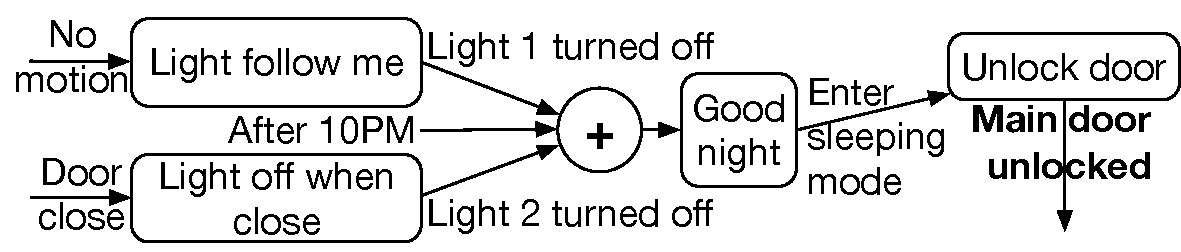
\includegraphics[width=3.4in]{violation_example}
				%\vspace{-0.06in}
		\caption{Example violation due to bad app interactions.}
        \label{violation_example}
    \end{subfigure}\\
    \vspace{0.03in}
    \begin{subfigure}[t]{3.6in}
        \centering
        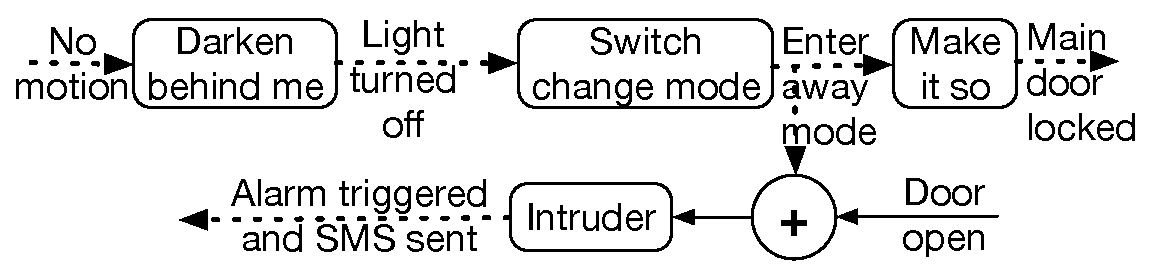
\includegraphics[width=3.6in]{device_failure}
				%\vspace{-0.06in}
        \caption{Example violation due to a device failure. Dotted arrows are
expected events that do not occur due to the failure of the motion sensor.}
		%\vspace{-0.1in}
        \label{device_failure}
    \end{subfigure}
    \caption{Violation examples: boxes depict apps and high level abstractions are
shown for inputs/outputs.}
    \label{violationexamples}
%\vspace{-0.30in}
\end{figure}

\begin{table*}[!tb]
\scriptsize
\ssp
\caption{Verification result of ContexIoT's malicious apps.}
\label{ContexIoT_apps}
\centering
{
\begin{tabular}{| c | p{1.8cm} | p{6.5cm} | p{3.9cm} |}
\hline
{\bf No.} & {\bf App's Name} & {\bf Malicious functions} & {\bf Violated properties}\\
\hline
1 & Battery Monitor & When the motion sensor detects that nobody is at home, the app would unlock the door. If the motion sensor detects that the user comes, the app would lock the door again. & The main door is unlocked when no one is at home\\
\hline
2 & Bon Voyage Repackage & When all people leave home, the app would notify the attackers via http post. & Information leakage (The command \textit{httpPost} is executed)\\
\hline
3 & Fake Alarm & The app triggers a fake CO detecting event. & Using security-sensitive command (generated CO detecting event)\\
\hline
4 & Leaking Info & The app would strobe the light when there is nobody home to signal the attacker. When user comes home (the motion sensor detects motion), the light stops strobing. & A light is turned on when no motion is detected and nobody is at home\\
\hline
5 & Water Valve &  The app does not let the user pull out the water until he pays the ransom money. & When smoke is detected, a water valve switch is turned off\\
\hline
6 & Fire Alarm & The app sends http post to the attacker periodically to get the attacker's command by http response. If the attacker's response is true, it would trigger a false alarm to annoy the users. & An alarm sirens when smoke is not detected\\
\hline
7 & Powers Out Alert & If the battery of the lock runs out, the app would not send message to the user about the low battery. Instead, it sends the message to the attacker so that the attacker could break in easily. & Information leakage (The command \textit{httpPost} is executed)\\
\hline
8 & Smoke Detector & The app sends http post to the attacker to get the dynamic command. The attacker could add the \textit{unsubscribe()} to the response so that he could disable the alarm \textit{subscribe}. & Using security-sensitive command (\textit{unsubscribe} is executed)\\
\hline
9 & Presence Sensor & The PresenceSensor sends the signal to the malicious light that there is nobody home. The malicious light start to use side channel to tell the MaliciousCameraIPC. The MaliciousCameraIPC receives this signal and sends it to the attacker. & A light is turned on when nobody is at home\\
\hline
\end{tabular}
}
\end{table*}


\textbf{Market apps with expert configurations}:
Table~\ref{market_apps} summarizes the results from our first set of experiments in the absence of device and communication failures.
The apps in parenthesis {\color{black} jointly cause} a violation. We find 38 violations of 11 properties,
some of which can be very dangerous from a user's perspective.
For example, there is violation where ``The main door is unlocked when people are sleeping at night'', which involves 4 apps.
%The format of the verification log is the same as that shown in Figure \ref{verificationlog}.
The interactions between the apps that lead to this violation is shown in Figure~\ref{violation_example}:
when lights are turned off at night a mode change is initiated by the \texttt{Good Night} app,
which in turn causes the unsafe action of unlocking the main door by the \texttt{Unlock door} app.

Device/communication failures cause violations of 9 additional properties with some dangerous cases.
One such case is showcased in Figure~\ref{device_failure}.
{\color{black}When people leave home, the \texttt{Make it so} app should automatically lock the entrance door;
however, due to the failure of the motion sensor, the \texttt{Make it so} app is not triggered and thus, the door is left unlocked.
Moreover, this failure also causes {\em NO} notification to be sent to law enforcement upon physical intrusion.}
%Here, a motion sensor failure causes subsequent actuations to fail even when no one is at home (lights are left on, and the door is left unlocked). This in turn fails to cause a notification to be sent to law enforcement upon physical intrusion.
An alarming discovery is that none of the analyzed apps check if the commands sent to the actuators
were actually carried out (which might not be the case if the device has failed).

\begin{comment}
{
as follows: (1) the \textit{inactive} event is generated for the livRoomMotion (no one present), which then updates its state and event queue, and notifies its subscriber {\color{black} app}; (2) the event handler of
the {\color{black} subscriber app}  \textit{Light Follows Me} is triggered and the command \textit{off} is sent to livRoomBulbOutlet, which subsequently updates its state and event queue, and notifies its subscriber; (3) the event \textit{closed} is generated for the bedRoomDoorContact, which then updates its state and event queue, and notifies its
own subscriber app; (4) the event handler of the app  \textit{Light Off When Close} is triggered and the command \textit{off} is sent to bedRoomBulbOutlet, which subsequently updates its state and event queue, and notifies its
subscriber app; (5) the event handler of the app \textit{Good Night} is triggered and the command \textit{mode} with value \textit{Sleeping} is sent to location, which subsequently updates its state and event queue, and notifies its subscriber app; (6) the event handler of the app \textit{Unlock Door} is triggered and the command \textit{unlock} is sent to mainDoorLock, which subsequently updates its state and event queue, and notifies its subscriber {\color{black} app}; (7) the event handler of the app \textit{Change Mode on Unlock} is triggered and the command \textit{mode} with value \textit{Home} is sent to location, which subsequently updates its state and event queue, and notifies its subscriber {\color{black} app}; (8) the event handler of the app \textit{Make It So} is triggered and the command \textit{on} is sent to TVOutlet and livRoomBulbOutlet, which subsequently update their states and event queues, and notify their subscriber {\color{black} apps}.
%\zhiyun{I'll simplify the description.}
}
\end{comment}

%{\color{black} A careful walk through of the above indicates that there are two violations: (i) the mainDoorLock's state is \textit{unlocked} when location mode is changed to \textit{Sleeping} and (ii) the TVOutlet's state is \textit{on} and livRoomBulbOutlet's state is \textit{on} when location mode is changed to \textit{Sleeping}.
%\zhiyun{careful walk though sounds like the result has to be manually analyzed. I think we should say that the two violations are automatically detected in the beginning and then just explain how model checking detected it.}}
%\krish{Do you mean -- unlocked "when" the location mode changes to Sleeping ? - and, on "when" the location mode is changed to sleeping?}


%At 10:00PM, when there is no motion in the living room, \textit{Light Follows Me} turns off all the lights in the living room. The home user goes into the bedroom and closes the door; thus, \textit{Light Off When Close} turns off the lights in the bedroom. After 30 minutes, \textit{Good Night} changes location mode to \textit{Sleeping} since all monitored lights are off and all motion sensors are inactive. On location mode change, \textit{Unlock Door} wrongly unlocks the main door, which triggers the \textit{Change Mode on Unlock} to change location mode to \textit{Home}. Since location mode is set to \textit{Home}, \textit{Make It So} restores the status of the house at \textit{Home} mode, \textit{i.e.}, it turns on the TV and all the lights in the living room. Apparently, we have three violations: (i) The main door is unlocked when people are sleeping at night, (ii) The location mode is wrongly set to \textit{Home}, and (iii) The TV and some lights are turned on when people are sleeping at night.

\textbf{Market apps with non-expert configurations}:
%Based on the previous experiment with market apps, we created 10 groups of apps with high dependency, and asked several students in our Computer Science Department to configure the apps. Each group had about five apps and was configured by seven students (\textit{i.e.}, each group had seven different configurations).
The verification results from the second set of experiments are in Table~\ref{user_market_apps} and Table~\ref{user_market_apps1}.
From 10 groups of apps with 70 configurations,
we find 97 violations of 10 properties.
For example, the property ``An AC and a heater are both turned on'' is violated by 21 configurations across 5 groups.
Note that in some configurations multiple properties are violated
and thus, the number of violations is more than the number of configurations.
%in which violation ratio is the number of configurations having violation over total number of configurations (\textit{i.e.}, seven).
\begin{comment}
{
The results indicate that there are four main causes of violations listed below.
For each, we provide an example.
\squishlist
\item {\em Bad app logic}: For example, the app \textit{Big Turn On} turns on configured devices when user touches the app. However, it also does the same when location mode changes. This is one of the causes of violations in group \#1.
\item {\em Too many configuration options}: There are 10 devices {\color{black} that
are controlled by} the \textit{switch} capability (e.g., light, TV, AC, heater, and microwave).
When configuring the app \textit{The Big Switch}, which turns on {\color{black} a set of devices}, when a specific switch is turned on, 3 out of 7 students choose both the heater and the AC. This configuration caused a violation viz., the \textit{AC and heater are both turned on}.
\item {\em Conflicting functionalities of apps}: Consider the conflicting pair of apps viz., \textit{Brighten Dark Places}, which turns on a light when a contact sensor is open and the space is dark, and \textit{Let There Be Dark!}, which turns off a light when a contact sensor is open and turns the light back on when it is closed
(both are present in a group presented to the volunteers). Six out of 7 volunteers configured the same devices for these two apps, which caused conflicting command violations.
\item {\em Bad app description}:
%In addition to the \textit{Unlock Door} app explained earlier, the \textit{Virtual Thermostat} app is another example.
\thomas{When the \textit{Virtual Thermostat} app said} ``select heater or air conditioner outlet(s)" -- the volunteers did not realize what that meant -- and ended up turning both on when an event (temperature change) occurred (recall \S~\ref{overview} for more details)
%The description of this app is ``\textit{Control a space heater or window air conditioner in conjunction with any temperature sensor, like a SmartSense Multi.}", and the text description when asking users to select devices is ``\textit{Select the heater or air conditioner outlet(s)...} ". Five out of 7 students {\color{black} configured the app to control both both AC and heater} which causes the violation wherein both \textit{an AC and a heater are both turned on}. \zhiyun{I don't really understand this example. Basically the user is not supposed to input both AC and heater?}
\squishend
}
\end{comment}

\begin{comment}
{
\begin{figure}[b]
    \centering
    \begin{subfigure}[t]{3.0in}
        \centering
        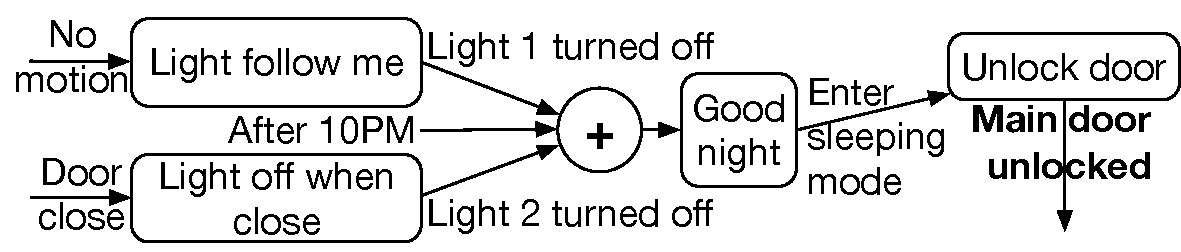
\includegraphics[width=2.8in]{violation_example}
                                \vspace{-0.06in}
                \caption{Example violation due to bad app interactions.}
        \label{violation_example}
    \end{subfigure}\\
    \vspace{0.03in}
    \begin{subfigure}[t]{3.2in}
        \centering
        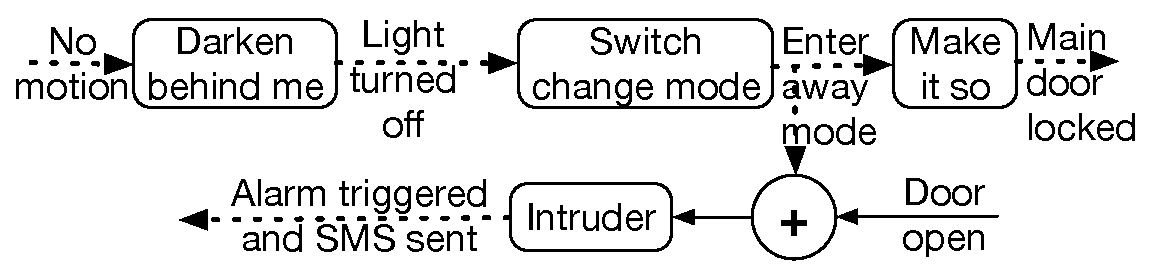
\includegraphics[width=2.8in]{device_failure}
                                \vspace{-0.06in}
        \caption{Example violation due to a device failure. Dotted arrows are
expected events that do not occur due to the failure of the motion sensor.}
                \vspace{-0.1in}
        \label{device_failure}
    \end{subfigure}
    \caption{Violation examples: boxes depict apps and high level abstractions are
shown for inputs/outputs.}
    \label{violationexamples}
\vspace{-0.25in}
\end{figure}
}
\end{comment}


% {\color{black}\sys discovered many serious safety violations, which can be induced by attackers via luring users to install malicious apps (\eg, \texttt{Unlock door} in Figure~\ref{violation_example}) or jamming the report of the motion sensor in Figure~\ref{device_failure}.}
%\vspace{-0.13in}
\section{Violation Attribution}
\sys attributes {\em all} of the ContexIoT's malicious apps~\cite{Jia:contexiot} correctly when each is independently considered
with violation ratios of 100 \% (recall \S\ref{outputanalyzer}). {\color{black}As shown in Table \ref{ContexIoT_apps},}
two apps violated the information leakage property as the command \textit{httpPost} was executed;
two apps violated the ``using security-sensitive command property",
\ie, they generated fake carbon monoxide detection events and an \textit{unsubscribe} is executed;
the remaining 5 apps violated safety properties in the physical space,
\eg, \textit{a main door is unlocked when no one is at home} and, \textit{when smoke is detected, a water valve switch is turned off}.
From among the 11 market apps, 6 were detected with a 100\% violation ratio,
both when verified independently and in conjunction with other apps; they were thus attributed as bad apps.
The remaining were attributed to cause violations (with 70\% or lower violation ratio)
due to bad configurations 
(there existed safe configurations with no violations).

%\vspace{-0.15in}
\section{Scalability}
\begin{comment}
{
\textbf{Runtime}: In all of the experiments we did, the verification halted within a second whenever a violation was present (and
discovered). When no violation was detected, the verification time (of the group from the user study alluded
to before) increases exponentially when the number of generated events increase from 6 to 11, as shown in table \ref{verificationtime}. {\color{black} According to the description in Table \ref{verificationtimesetup} of the devices used in this experiment, we have $(3*2)*(1*2)*(1*5)*(1*3)=180$ options to select a physical event for a sensor at each iteration in Algorithm \ref{alg:smarthingprocess}. If we generate 10 physical events, there are $180^{10}$ permutations of the input sequences. Moreover, each physical event may trigger some new cyber events. This explains the increasing trend of the runtime. Since we ran the experiments in a laptop with limited computing resources, we used 10 events in all of the experiments we did. One may run the experiments with much more generated events in super computing machines or in the cloud to increase the verification coverage. Note that all of the violations we found were detected with just several generated events (\textit{e.g.}, 2 or 3) or even a single event in many cases.}
%\krish{What is the take away here?  It seems abrupt and the reader is left hanging.}
}
\end{comment}

Table~\ref{scalability} shows the scalability benefits of our app dependency analyzer in the above experiments with 150 market apps.
In this table,
``\textit{Original Size}" is the total number of event handlers of a group and
``\textit{New Size}" is the number of event handlers of the largest related set after running the \textit{App Dependency Analyzer} module.
On average, \textit{App Dependency Analyzer} reduced the problem size by a factor 3.4x.


\begin{table}[t]
\ssp
\scriptsize
   %\vspace{-0.13in}
    \caption{Scalability with dependency graphs}
	%\vspace{-0.15in}
    \centering
		%\vspace{-0.05in}
        \label{scalability}
		{
		\begin{tabular}{| c | c | c | c |}
		\hline
		\bf Group & \bf Original Size & \bf New Size & \bf Scale Ratio\\
		\hline
		1 & 37 & 11 & 3.4\\
		\hline
		2 & 27 & 5 & 5.4\\
		\hline
		3 & 34 & 23 & 1.5\\
		\hline
		4 & 30 & 12 & 2.5\\
		\hline
		5 & 42 & 19 & 2.2\\
		\hline
		6 & 34 & 6 & 5.7\\
		\hline
		\multicolumn{3}{|c|}{\textbf{Mean scale ratio}} & \textbf{3.4}\\
		\hline
		\end{tabular}
		}
%\vspace{-0.15in}
\end{table}

\begin{table}[t]
\ssp
\scriptsize
   %\vspace{-0.13in}
    \caption{Runtimes with concurrent and sequential design.}
		%\vspace{-0.05in}
		\centering
        \label{designruntime}
		{
		\begin{tabular}{| c | c | c |}
		\hline
		\bf Number of events & \bf Concurrent & \bf Sequential\\
		\hline
		1 & 1s &  1s\\
		\hline
		2 & 56.5s & 1s\\
		\hline
		3 & 139m & 1s\\
		\hline
		4 & forever &  1s\\
		\hline
		5 &  &  1s\\
		\hline
		6 &  &  4.2s\\
		\hline
		7 &  &  16.3s\\
		\hline
		\end{tabular}
		}
%\vspace{-0.15in}
\end{table}


\begin{table}[tb]
\scriptsize
\ssp
\caption{Verification time vs. number of events.}
%\vspace{-0.1in}
\centering
\label{verificationtime}
{
\begin{tabular}{| c | c | c | c | c | c | c |}
\hline
\bf Number of events & 6 & 7 & 8 & 9 & 10 & 11\\
\hline
\bf Verification time & 6.61s & 50.9s & 396s & 49.83m & 5.89h & 23.39h\\
\hline
\end{tabular}
%\vspace{-0.2in}
}
\end{table}

\begin{comment}
{
\begin{table}[!h]
\scriptsize
\caption{Scalability of dependency graph with market apps.}
\label{scalability}
\centering
\begin{tabular}{| c | c | c | c |}
\hline
Group & Original Size & New Size & Scale Ratio\\
\hline
1 & 37 & 11 & 3.4\\
\hline
2 & 27 & 5 & 5.4\\
\hline
3 & 34 & 23 & 1.5\\
\hline
4 & 30 & 12 & 2.5\\
\hline
5 & 42 & 19 & 2.2\\
\hline
6 & 34 & 6 & 5.7\\
\hline
\multicolumn{3}{|c|}{\textbf{Mean scale ratio}} & \textbf{3.4}\\
\hline
\end{tabular}
\vspace{-0.4in}
\end{table}
}
\end{comment}

%\vspace{-0.13in}
\section{Concurrent vs. Sequential}
%\krish{What two bad groups ? We never said anything here. Can we say, "All bad configurations that were detected, were identified very quickly (within X seconds) by both approaches." Don't think example is needed here.}
%Both of the design approaches detected all of the violations of the two bad groups. Two violations of (Auto Mode Change, Unlock Door) are (i) \textit{a door is unlocked when no one is at home} and (ii) \textit{a door is unlocked when the app is not touched}. One violation of (Brighten Dark Places, Let There Be Dark) is a conflicting command (on \textit{v.s.} off).
Model checkers using both concurrent and sequential design detected all violations
within 1 second. Table~\ref{designruntime} shows the runtimes of the two models with
a good group of apps (\textcolor{black}{2 apps and 7 devices}), which does not violate any property.
We see that sequential design significantly reduces the runtime of the verification.
Note that \textit{forever} means the experiment ran for a week and then was forced to stop.
Moreover, we also verified the runtime of our sequential approach with a much bigger system,
which comprises of 5 related apps and 10 devices and does not have any violation.
{\color{black}As shown in Table~\ref{verificationtime}}, the verification time for 10 events is about 5 hours,
which is quite reasonable for a laptop with limited computing resources.
%We point out that in all of the experiments we did, the violations were detected within {\color{black}several seconds}.
%Recall that as demonstrated in our volunteer experiments,
%humans cannot easily detect unintended bad consequences of complex app interactions
%even given time.
%\vspace{-0.13in}
\chapter{Discussion}
{\color{black}
\section{Application to other IoT Platforms}
For ease of exposition, our narrative integrated some aspects of
implementation specific to SmartThings, when describing the design of \sys. Conceptually,
the design of \sys applies to other IoT platforms. To illustrate, given its recent popularity we choose IFTTT (IF This Then That~\cite{iftttpage})~\cite{Liang:2015:SBI:2737095.2737115,Ur:2016:TPW:2858036.2858556,Mi:2017:ECI:3131365.3131369} to show that this is the case. IFTTT is a task automation platform for IoT deployments. An IFTTT rule (also called applet) comprises of two main parts: ``Trigger Service'' (This) and ``Action Service'' (That). To apply \sys to IFTTT, most of the modules (\ie, \textit{App Dependency Analyzer}, \textit{Model Generator}, and \textit{Output Analyzer}) can be reused almost as is; the relatively big change will be in the \textit{Translator}.

%Top IoT-related trigger services include Amazon Alexa~\cite{Amazon:alexa}, \href{https://nest.com/}{Nest Thermostat}, and \href{https://assistant.google.com/}{Google Assistant}; \href{http://www2.meethue.com}{Philips Hue}, Samsung SmartThings~\cite{Samsung:smartthings}, and \href{http://www.belkin.com/us/F7C030/p/P-F7C030/}{WeMo Smart Plug} are among popular IoT-related action services ~\cite{Mi:2017:ECI:3131365.3131369}. Xianghang Mi \etal ~\cite{Mi:2017:ECI:3131365.3131369} develop a crawler to fetch a large number of published applets from IFTTT website and save them to a \textit{recipes.json} file.

\textbf{\em IFTTT to Java Translator}: We use the crawler of \cite{Mi:2017:ECI:3131365.3131369} to fetch the published applets from IFTTT website into a \textit{json} file. We then developed an \textit{IFTTT Handler} in Java based on the \textit{org.json.simple} package to extract the subscribed device and event from the trigger service, and the controlled device and expected command from the action service of each IFTTT rule. {\color{black} The translation is relatively simple.} Each rule is considered as an app, which has only a single event handler, in \sys and is translated into a Java class. Each event handler (\ie, a Java method) has only a single instruction (\ie, the expected command); the subscribed device and controlled device become class fields. Even though the technical details of \textit{IFTTT Handler} are somewhat different from \textit{SmartThings Handler}, the translation procedures are very similar (\eg, all Java objects and grammars are exactly the same).

\textbf{\em Minor changes in Model Generator}: Each service is map-ped onto (modeled as) a sensor device(s) or an actuator device(s). We have modeled 8 popular IoT-related services based on the events/actions they provides on the IFTTT website. For example, Amazon Alexa~\cite{Amazon:alexa} and \href{https://assistant.google.com/}{Google Assistant} are modeled as sensor devices; \href{https://nest.com/}{Nest Thermostat} is modeled as an actuator device. {\color{black} The difference is that Samsung SmartThings 
inherently provides handlers for several kinds of devices (\eg, outlet, lock, motion sensor, and contact sensor)}. The change needed is to add more device types to the collection of modeled devices.

We have validated our basic IFTTT prototype implementation with 10 IoT rules/applets (from \cite{iftttpage}) assuming that all of these rules are installed in a smart home. We perform limited experiments and as shown in Table~\ref{iftttresults} (hyperlinks to a rule --e.g., rule \#1 -- can be seen by clicking on the rule), we find 7 violations of 4 unsafe physical states.
\begin{table}[tb]
\scriptsize
\caption{Verification results with IFTTT rules.}
%\vspace{-0.12in}
\label{iftttresults}
\centering
{\begin{tabular}{| p{10cm} | p{4cm} |}
\hline
{\bf Violated properties} & {\bf Related rules}\\
\hline
Siren/strobe is not activated when intruder (\ie, motion) is detected & (\href{https://ifttt.com/applets/156916p-strobe-my-smartthings-siren-if-category-1-hurricane-winds-are-nearby}{rule \#1}, \href{https://ifttt.com/applets/342118p-alexa-tells-smarthings-to-turn-off-siren}{rule \#4}), (\href{https://ifttt.com/applets/260978p-motion-siren-on}{rule \#3}, \href{https://ifttt.com/applets/342118p-alexa-tells-smarthings-to-turn-off-siren}{rule \#4})\\
\hline
Siren/strobe is activated when no intruder is detected & (\href{https://ifttt.com/applets/342120p-alexa-tells-smarthings-to-turn-on-siren}{rule \#2})\\
\hline
The main/front door is unlocked when no one is at home & (\href{https://ifttt.com/applets/115638p-let-me-in-checkin-with-a-hashtag-to-unlock-your-door}{rule \#5}), (\href{https://ifttt.com/applets/348905p-alexa-unlock-the-frond-door}{rule \#6})\\
\hline
A phone call is not triggered when intruder is detected & (\href{https://ifttt.com/applets/419985p-disarm-your-arlo-camera-network-with-alexa}{rule \#7}, \href{https://ifttt.com/applets/413211p-if-arlo-detects-motion-call-my-phone}{rule \#10}), (\href{https://ifttt.com/applets/raiAMZLh-tell-google-assistant-to-disarm-your-arlo}{rule \#8}, \href{https://ifttt.com/applets/413211p-if-arlo-detects-motion-call-my-phone}{rule \#10})\\
\hline
\end{tabular}}
%\vspace{-0.27in}
\end{table}
}

\section{Limitations}
While our prototype of \sys has been shown to be very effective in
identifying bad apps and unsafe configurations, it has the following limitations.
%
{\em First,} the \spin model checker has a predefined threshold for the size of Promela code
(and cannot handle a file size greater than this).
Depending on apps' source code sizes and dependencies among the apps, \sys can handle a system with about 30 apps.
We assume that users are unlikely to have many more than this today and will investigate further scalability in the future.
%{\em Second},  Groovy has many built-in utilities and SmartThings has a lot of APIs and supports a wide range of device types. However, we have just incorporated the most common features of SmartThings and Groovy (\textit{e.g.}, \texttt{find}, \texttt{findAll}, \texttt{each}, \texttt{collect}, \texttt{first}, $+$ on list types, and \texttt{map}), which are widely used by most smart apps. One can handle the remaining features but this will incur more engineering effort which we leave for future work.
%{\color{violet}{\em Second}, one can apply \sys to other hub-based IoT platforms ~\cite{Vera:homecontroller,Intel:smartbuildings, Logitech:harmony,Microsoft:iot} but this will incur more engineering effort to replace the \textit{Translator} module with a new one, which translates from a language other than Groovy into Java; we leave this effort for future work.}
%
{\em Second}, we require smart apps to explicitly subscribe to specific devices they want to control
and cannot handle smart apps that dynamically discover devices and interact with them.
Such apps are very dangerous since they can control any device without permissions from users.
Identifying such apps and ensuring that they do not compromise the physical state is beyond the scope of this effort.
%
{\em Third}, in Algorithm \ref{alg:smarthingprocess}, we let the model checker enumerate all possible permutations of the event types;
thus, it may consider scenarios that are unlikely to happen in the real world
(\eg, the temperature is set to a minimum value in the first iteration and set to a maximum value in the second one).
However, we include these scenarios to catch bad or malicious apps.
If such scenarios can be eliminated, the state explosion issue can be further mitigated.
%
{\em Fourth}, we do not explicitly model the behavior of the physical environment after an actuator executes a command
(\eg, the system temperature should increase after a heater is turned on).
However, such physical changes are implicitly covered by the way the model checker \textcolor{black}{exhaustively} verifies a system.
%{\em Sixth}, one may claim that legitimate apps can use the SmartThings APIs (\textit{e.g., httpPost}) to send some crash info back to the server. However, users may have their own reasons to disallow such operations to prevent private information leakage. We let the user decide which properties their IoT system should satisfy. 
%{\em Finally}, to mitigate the impact of device failures on the system, after sending a command to an actuator, a smart app needs to check if the actuator is in the expected state. If not, the smart app should notify users of this incident via SMS/Push message.}
%To illustrate, let us consider a system that consists of five devices and each device has two types of events. For the sake of simplicity, we ignore the two event types $sunriseTime$ and $sunsetTime$. At each iteration in the Algorithm \ref{alg:smarthingprocess}, there are 10 options to select an event type that is to be generated. If we generate $10$ events, there will be $10^{10}$ permutations of the events, \textit{i.e.}, there will be $10^{10}$ ways to generate 10 events. In verification mode, a model checker will enumerate all of the permutations to exhaustively verify the system. Therefore, the event sequent ``a heater is turned on" and then ``the system temperature is increased" is just one of the permutations.
%\krish{I do not get the example -- do we really need it?  It seems to exemplify the state space explosion problem -- and not focused on the fact that the physical change is captured implicitly. I would remove.}
{\color{black}{\em Fifth}, the G2J Translator currently does not
support heterogeneous collections (\eg, a list, array, or map that stores entries of different types) and
dynamic features (\eg, overloading operator and generic data types). Note that most of the
SmartThings apps do not use these features.}


%\vspace{-0.12in}
\chapter{Related Work}
\label{sec:related}
%IoT systems have grown in popularity and have already hit the markets. Samsung's SmartThings \cite{Samsung:smartthings}, Apple's HomeKit \cite{Apple:homekit}, Google's Weave/Brillo \cite{Google:weave}, Vera's Smart Home Controller \cite{Vera:homecontroller}, and Intel's Smart Buildings \cite{Intel:smartbuildings} are among the most popular platforms. Third party apps to drive these systems are also proliferating and can enable diversity in usage and new features as they evolve. However, the safety of using such applications will have to be ensured to protect users. \sys addresses this issue.

%\noindent
\section{IoT Security} Current research on IoT security can be roughly divided into three categories that focus on devices \cite{Ronen2016:extended,Fisher:honeywellbug,Hesseldahl:hackereye}, protocols \cite{Fouladi2013,Ho2016:smartlock, Lomas:zigbeeflaw,Eyal:iotworm}, and platforms. There have been efforts addressing information leakage and privacy~\cite{Christoph2015,Judson2017:rar,Sha2017,Bertino:2016:ITS:3023158.3013520,Yuchen2017,217632}, and vulnerabilities of firmware images \cite{Costin:analysis}.
Fernandes \textit{et al.}, have recently reported security-critical design flaws in the IoT permission model that could expose smart home users to significant harm such as break-ins~\cite{Earlence:smarthomesecurityanalysis}. 
%To address these,  they propose FlowFence \cite{Earlence:flowfence}, a system that requires smart apps  to declare their intended data flow patterns. It then explicitly embeds some extra code into the smart app's structure to block undeclared flows. ContexIoT \cite{Jia:contexiot}, provides contextual integrity by supporting fine-grained context identification for sensitive actions, to help users perform effective access control. {\color{black}ProvThings~\cite{Wang:ProvThings} performs code instrumentation of apps and device handlers and audit system activities at run time.}
%SmartAuth~\cite{203866} generates a user interface \textcolor{black}{that facilitates educated authorizations based on the app's functions and operations.}
{\color{black}To address these, several efforts~\cite{Earlence:flowfence,Jia:contexiot,203866,Wang:ProvThings} have proposed modifications} to a smart app's source code and the platform, 
to enforce good behaviors of smart apps at run time. In contrast, our work statically identifies
possible violations of given 
physical/cyber safety properties of IoT systems without requiring any app modifications. 
%Specifically we seek to identify interactions among installed smart apps, behaviors of
%malicious apps, and device failure triggers, that cause bad physical states . 

%\noindent
\section{Model Checking}
%Model checking, a formal verification technique for assessing functional properties of information and communication systems, has been widely used by researchers across many areas \cite{Seth2016:smartgrid,Chen2013:contextual,Roya:networkprotocol,Sardar2016, Ali2013:ami, Ouchani2013:securityrisk}. This technique has also 
{\color{black}Model checking has
been used to verify system-level threats ~\cite{Mohsin2017:IoTChecker,Mohsin2017:IoTRiskAnalyzer,Mohsin2016:IoTSAT} and {\color{black}basic correctness properties~\cite{Liang:2015:SBI:2737095.2737115,190480,215955,Newcomb:2017:ICI:3133850.3133860}} of IoT systems.}
%IoTRiskAnalyzer \cite{Mohsin2017:IoTRiskAnalyzer} is a probabilistic model checking system 
%that takes a set of deployment configurations (\textit{e.g.}, IoT devices and their network), operational policies (\textit{i.e.}, the rules based on which the sensing data is processed and actuation commands are triggered), vulnerability exploitation scores of individual IoT components, and attacker capabilities as inputs. It then 
%that generates system and threat models to capture the risk exposure of each input configuration. 
%IoTSAT \cite{Mohsin2016:IoTSAT} utilizes Satisfiability Modulo Theories (SMT) \cite{deMoura:SMT} to formally model the generic behavior of IoT systems. 
%based on device configurations, network topologies, user policies and IoT-specific attack surface. The model is then used to measure system's resilience against potential attacks and identify threat vectors and specific attack techniques. 
%SIFT \cite{Liang:2015:SBI:2737095.2737115} takes app's rules as inputs and uses a synthesis engine to generate code that is specific to the deployment environment. SIFT then uses white-box model checking to verify that synthesized IoT apps do not violate safety policies. {\color{black}Soteria~\cite{215955} and DeLorean~\cite{Delorean} use model checking to verify basic correctness properties of IoT systems.}
In contrast with these efforts, \sys targets developing a practical platform for ensuring
the physical safety of today's IoT systems. It not only addresses
the practical challenges (\eg, scale issues and making Groovy amenable to model checking) 
in identifying configurations that violate user properties relating to
the physical state, but also addresses robustness (failures) and security issues (malicious app attribution). {\color{black}Table \ref{table:comparison} shows what \sys offers compared to the most related recent systems.}

%\vspace{-0.13in}
\chapter{Conclusions}
%Unlike traditional cyber-systems, the IoT systems can be affected due to the compromise of 
%the physical functioning of actuators. 
Badly designed apps, undesirable interactions between installed apps and/or {\color{black}device/communication failures} can cause an IoT system to transition into bad states. In this paper, we design and prototype a framework \sys that 
uses model checking as a basic building block to identify causes for bad physical/cyber states 
and provides counter-examples to exemplify these causes.
\sys addresses practical challenges such as alleviating state space
explosion with model checking, and automatic translation of app code into a form
amenable for model checking. %and is applicable to today's IoT systems. 
Our evaluations show
%case its effectiveness by evaluating it with 150 smart apps in SmartThings' market place and 25 malicious apps created by ContexIoT \cite{Jia:contexiot}. 
that \sys \textcolor{black}{identifies many (sometimes complex) unsafe configurations}, 
and 
{\color{black}flags considered bad apps with 100\% accuracy.}




\nocite{*}
% \singlespacing
% \bibliographystyle{alpha}
\bibliographystyle{plain}
%\bibliographystyle{./bibtex/ACM-Reference-Format}
\bibliography{./bibtex/mybibfile}

\appendix



\end{document}
